\chapter*{\textbf{Capítulo IV: Análisis de Resultados}}
\label{ch:Resultados}
\addcontentsline{toc}{chapter}{\textbf{IV. Análisis de Resultados}}
\chead{Análisis de Resultados}
\setcounter{chapter}{4}
\setcounter{equation}{0}
\setcounter{figure}{0}
\setcounter{table}{0}

\section*{IV.1 Simulaciones}
\addcontentsline{toc}{section}{IV.1 Simulaciones}

\subsection*{IV.1.1 Determinación de candidatos a tránsitos}
\addcontentsline{toc}{subsection}{IV.1.1 Determinación de candidatos a tránsitos}

Para determinar la eficiencia de la metodología en la identificación de candidatos a tránsitos de exoplanetas, se utilizó el coeficiente de correlación de Pearson como medida de la calidad del ajuste. También evaluamos la distorsión de la curva de luz, debido a los diferentes métodos de filtrado, para esto calculamos la diferencia porcentual entre el parámetro $t_c$ de la simulación y los obtenidos mediante el ajuste.

Utilizando la base de datos de tránsitos simulados (véase III.3.1) y los ruidos simulados (véase III.2.3) se calcularon los coeficientes de correlación de 625 casos únicos (25 $\Delta F$ y 25 $t_{c}$).

Presentaremos los resultados por método de filtrado, y para los casos límites de ruido, es decir $SNR=10$ y $SNR=100$. Estos valores de SNR's son de antes de cualquier proceso de filtrado.

\subsubsection*{IV.1.1.1 Resultados del filtro de Fourier}
\addcontentsline{toc}{subsubsection}{IV.1.1.1 Resultados del filtro de Fourier}

Las figuras \ref{fig_correlaciones_fou_10} y \ref{fig_correlaciones_fou_100} muestran la correlación, entre el modelo y la curva filtrada con el filtro de Fourier, para curvas con $SNR=10$ y $SNR=100$ respectivamente. El color nos indica la media de los coeficientes de correlación ($C$), de los 100 ruidos con diferentes parámetros (véase III.2.3).

\begin{figure}
	\centering
		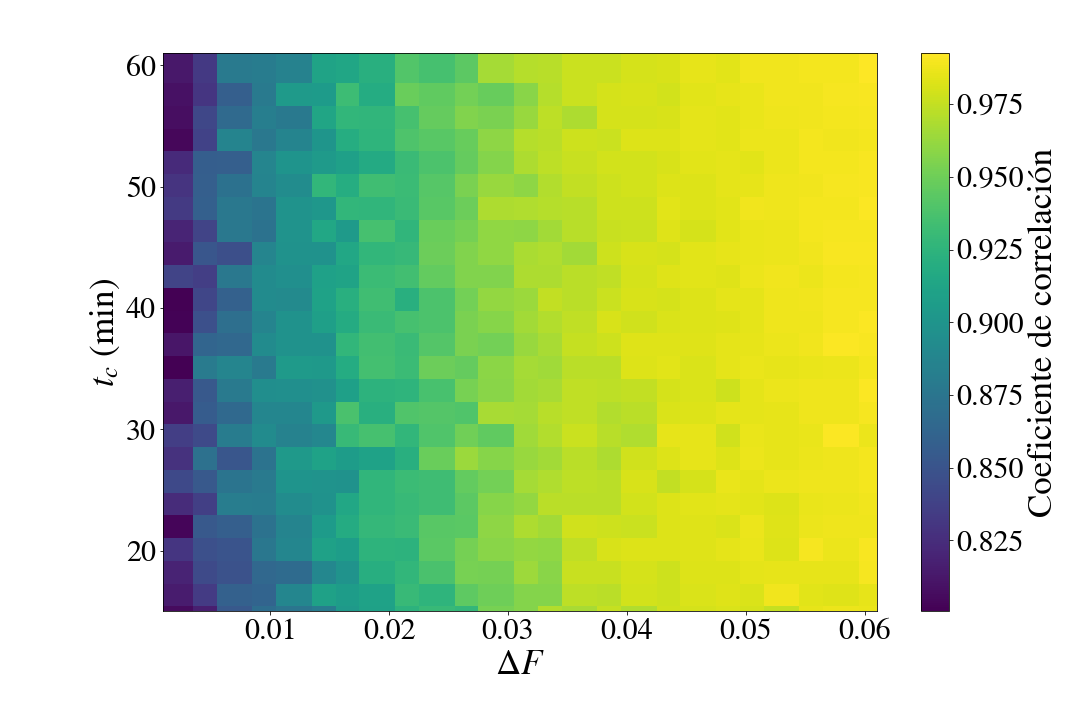
\includegraphics[max size={0.9\textwidth}{0.36\textheight}]{./figures/corrFourierSNR_10.png}
		\caption{Matriz de correlaciones de los parámetros $\Delta F$ y $t_{c}$ entre las simulaciones y los calculados después de aplicar el modelo del trapezoide a los datos filtrados utilizando Fourier. Estos resultados se obtuvieron a partir de curvas simuladas con una $SNR=10$.}
		\label{fig_correlaciones_fou_10}
\end{figure}

\begin{figure}
	\centering
		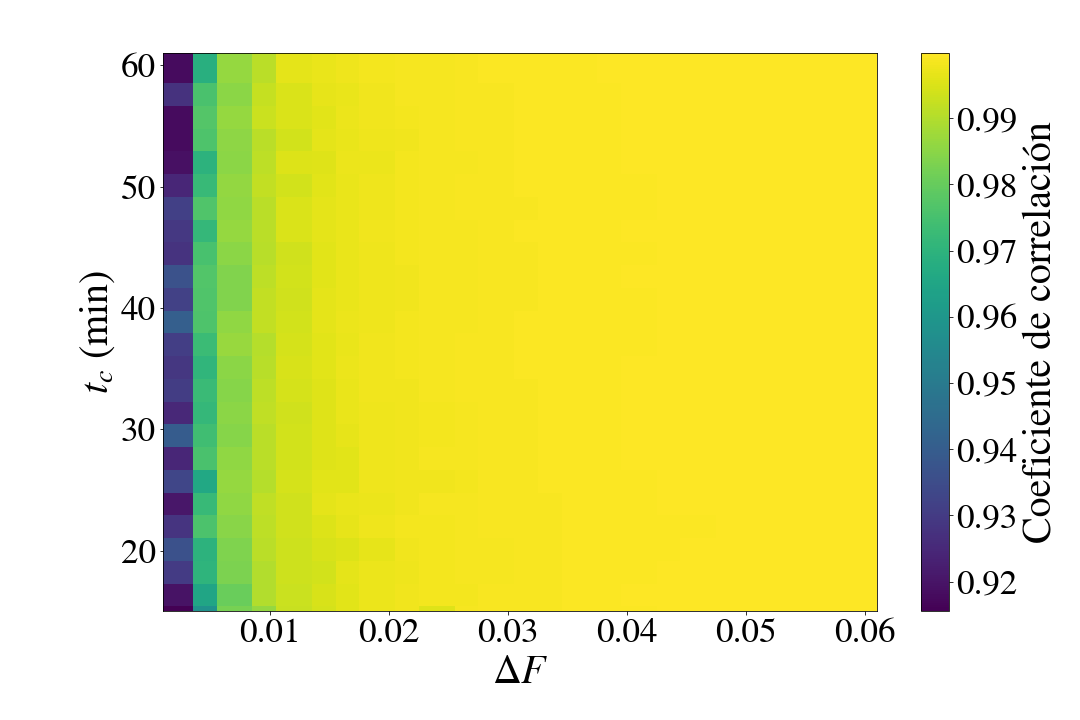
\includegraphics[max size={0.9\textwidth}{0.36\textheight}]{./figures/corrFourierSNR_100.png}
		\caption{Matriz de correlaciones de los parámetros $\Delta F$ y $t_{c}$ entre las simulaciones y los calculados después de aplicar el modelo del trapezoide a los datos filtrados utilizando Fourier. Estos resultados se obtuvieron a partir de curvas simuladas con una $SNR=100$.}
		\label{fig_correlaciones_fou_100}
\end{figure}

Estos resultados ayudan a saber que tipos de sistemas planetarios, podrían ser detectados utilizando esta metodología. También nos ayuda a definir la cota inferior para el coeficiente de correlación entre el modelo y la curva filtrada, para que esta, sea considerada como candidato a tránsito. Para el método de filtrado con Fourier, la cota inferior para el coeficiente de correlación es de $C \geq 0.85 $. 

Esta cota inferior se calculó a partir de un estudio de falsos positivos, donde se aplicó la metodología planteada en este trabajo, a curvas con solo ruido. De estos resultados, tomamos el coeficiente de correlación máximo $C_{max}$ y calculamos la cota inferior como: 

\begin{equation}
	C_{cota}= \dfrac{1+C_{max}}{2}
\end{equation}


Si analizamos la figura \ref{fig_correlaciones_fou_100}, vemos que para las curvas con $SNR=100$, todo el intervalo de valores de $\Delta F$ y $t_{c}$ (dentro de los límites, véase IV.2) tiene un valor de $C$ es mayor que la cota inferior. Esto significaría, que en principio seríamos capaces de detectarlos. Por otra parte, en la figura \ref{fig_correlaciones_fou_10}, vemos que para curvas con $SNR=10$ los tránsitos con $\Delta F < \sim 0.005$ no serían detectables.

Las figuras \ref{fig_diferencias_fou_10} y \ref{fig_diferencias_fou_100} muestran la diferencia porcentual entre $t_{c}^{Fit}$ y $t_{c}^{Real}$, que representan la duración de $t_{c}$ calculada mediante el ajuste y el valor real de la simulación respectivamente. El color nos indica diferentes valores de $\Delta F$. En la figura \ref{fig_diferencias_fou_10} se ilustra los resultados para una $SNR=10$ y los de $SNR=100$ en la figura \ref{fig_diferencias_fou_100}.


\begin{figure}
	\centering
		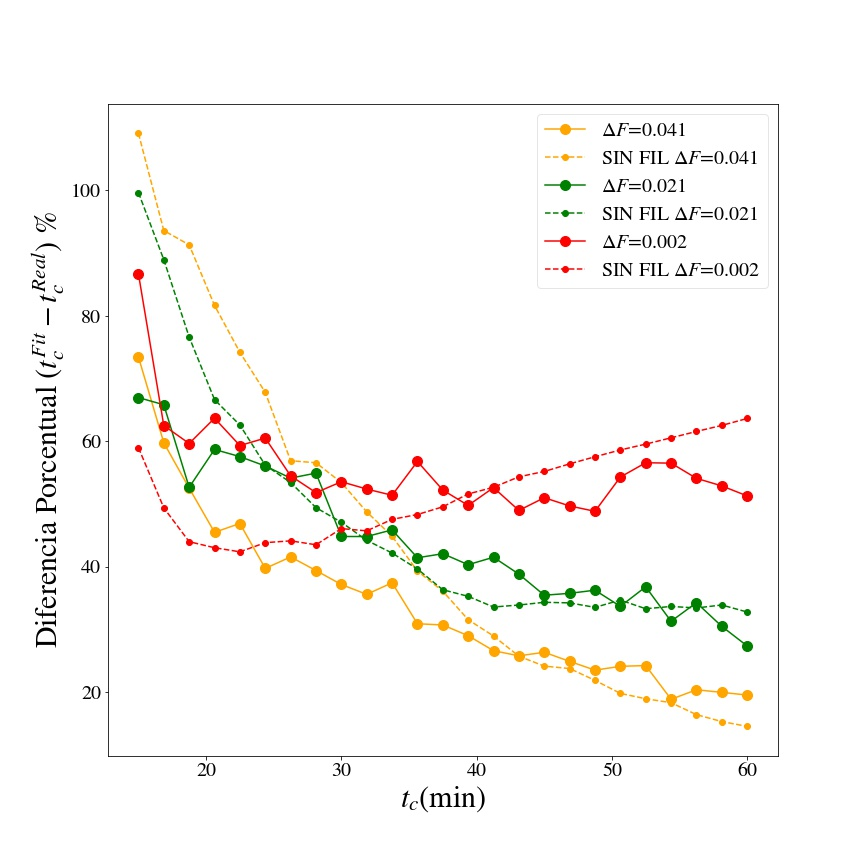
\includegraphics[max size={\textwidth}{0.9\textheight}]{./figures/Dif_SNR_10_Fourier.jpg}
		\caption{Las lineas sólidas representan la diferencia porcentual entre $t_{c}^{Fit}$ y $t_{c}^{Real}$ después de aplicar el modelo del trapezoide a los datos filtrados utilizando el filtro de Fourier. Las líneas punteadas representan la misma cantidad, pero obtenida aplicando el modelo del trapezoide a las curvas simuladas sin filtrar. El color representa diferentes valores de $\Delta F$, se utilizaron 4\%, 2\% y 0.2\% representados en amarillo, verde y rojo respectivamente. Estos resultados se obtuvieron a partir de curvas simuladas a las que se les insertó un ruido con una $SNR=10$.}
		\label{fig_diferencias_fou_10}
\end{figure}

\begin{figure}
	\centering
		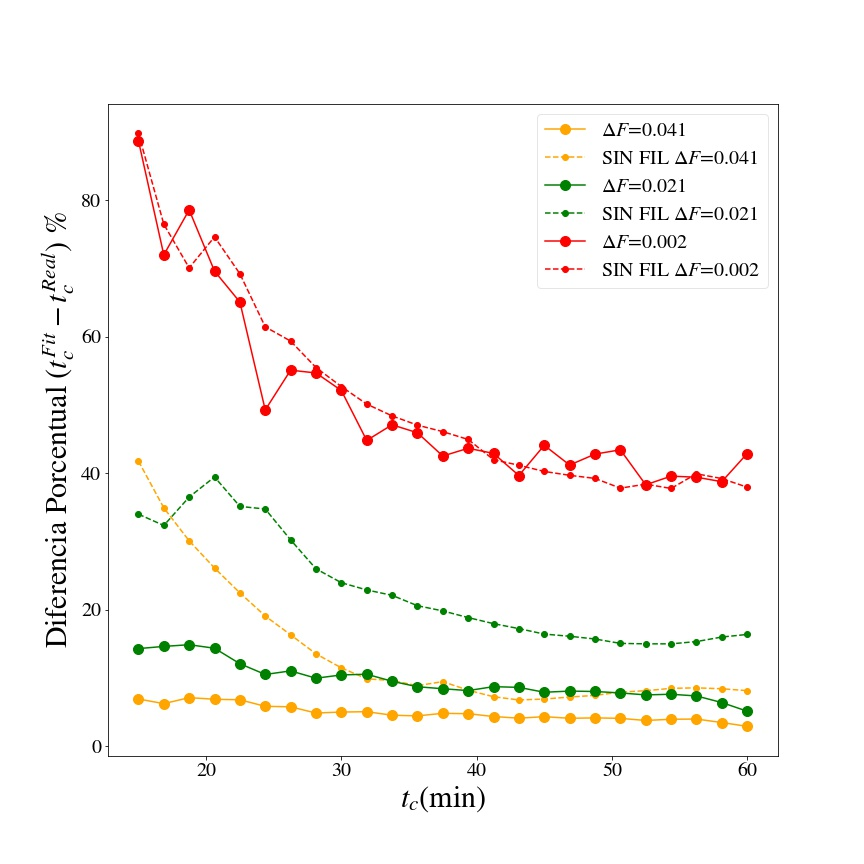
\includegraphics[max size={\textwidth}{0.9\textheight}]{./figures/Dif_SNR_100_Fourier.jpg}
		\caption{Las lineas sólidas representan la diferencia porcentual entre $t_{c}^{Fit}$ y $t_{c}^{Real}$ después de aplicar el modelo del trapezoide a los datos filtrados utilizando el filtro de Fourier. Las líneas punteadas representan la misma cantidad, pero obtenida aplicando el modelo del trapezoide a las curvas simuladas sin filtrar. El color representa diferentes valores de $\Delta F$, se utilizaron 4\%, 2\% y 0.2\% representados en amarillo, verde y rojo respectivamente. Estos resultados se obtuvieron a partir de curvas simuladas a las que se les insertó un ruido con una $SNR=100$.}
		\label{fig_diferencias_fou_100}
\end{figure}

Podemos observar que para tránsitos con una profundidad $\Delta F\, > 1\%$ y los $t_{c}$ más cortos (15-40 min) este método es más efectivo, fuera de estos rangos no se aprecia una diferencia significativa entre los resultados obtenidos sin aplicar filtrado y aplicándolo. En el caso de $SNR=10$ se aprecia como para el caso de $\Delta F=0.2\%$ en algunos casos, el ajuste sin filtrar dio mejores resultados, esto se debe a la deformación en los bordes de la curva debido a el filtrado de Fourier.


\subsubsection*{IV.1.1.2 Resultados del promedio móvil}
\addcontentsline{toc}{subsubsection}{IV.1.1.2 Resultados del promedio móvil}

De manera análoga, las figuras \ref{fig_correlaciones_mov_10} y \ref{fig_correlaciones_mov_100} muestran la correlación, entre el modelo y la curva filtrada con el promedio móvil, para curvas con $SNR=10$ y $SNR=100$ respectivamente. El color nos indica la media de los coeficientes de correlación ($C$), de los 100 ruidos con diferentes parámetros (véase III.2.3).

\begin{figure}
	\centering
		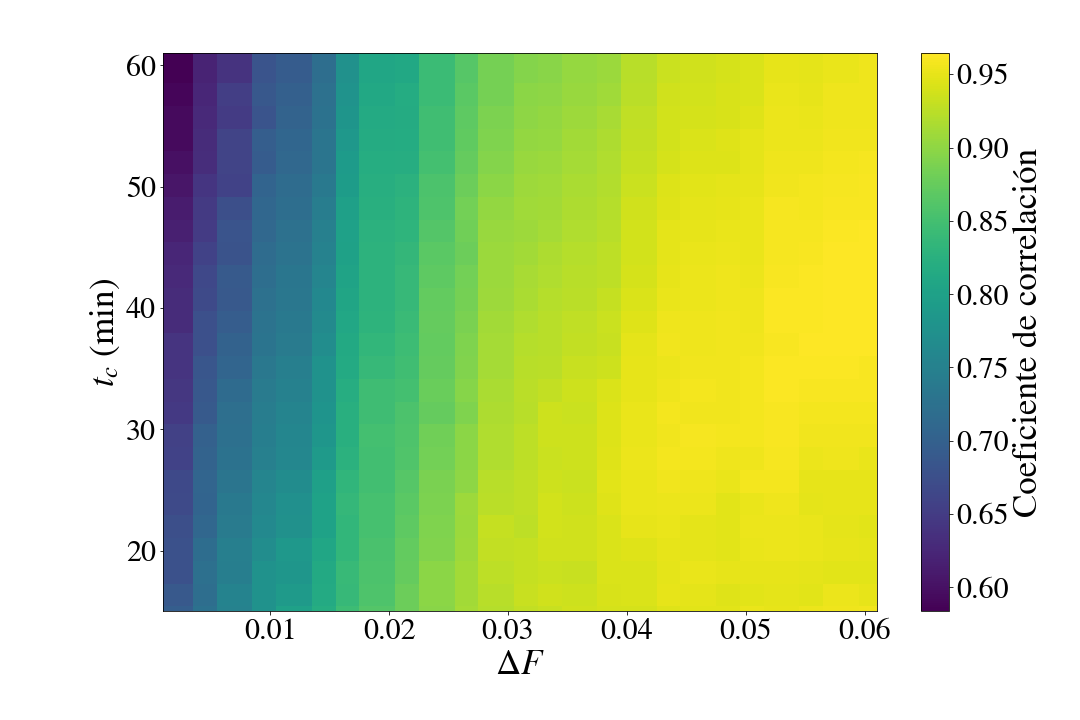
\includegraphics[max size={0.9\textwidth}{0.36\textheight}]{./figures/corrMovSNR_10.png}
		\caption{Matriz de correlaciones de los parámetros $\Delta F$ y $t_{c}$ entre las simulaciones y los calculados después de aplicar el modelo del trapezoide a los datos filtrados utilizando promedio móvil. Estos resultados se obtuvieron a partir de curvas con una $SNR=10$.}
		\label{fig_correlaciones_mov_10}
\end{figure}

\begin{figure}
	\centering
		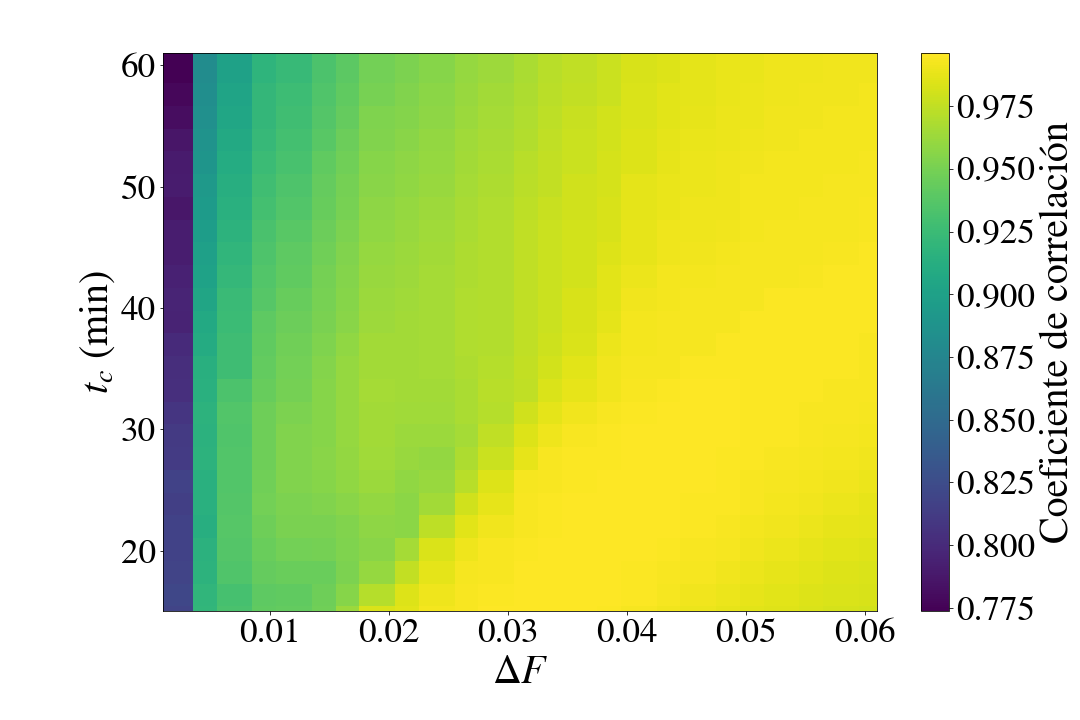
\includegraphics[max size={0.9\textwidth}{0.36\textheight}]{./figures/corrMovSNR_100.png}
		\caption{Matriz de correlaciones de los parámetros $\Delta F$ y $t_{c}$ entre las simulaciones y los calculados después de aplicar el modelo del trapezoide a los datos filtrados utilizando promedio móvil. Estos resultados se obtuvieron a partir de curvas con una $SNR=100$.}
		\label{fig_correlaciones_mov_100}
\end{figure}

Para el método de promedio móvil, la cota inferior para determinar una curva como candidata a tránsito es de $C \geq 0.84 $. Si analizamos la figura \ref{fig_correlaciones_mov_100}, vemos que para este método de filtrado, los valores de $C$ están en función de $\Delta F$ y más notablemente de $t_{c}$. 

Las figuras \ref{fig_diferencias_mov_10} y \ref{fig_diferencias_mov_100} muestran la diferencia porcentual entre $t_{c}^{Fit}$ y $t_{c}^{Real}$, que representan la duración de $t_{c}$ calculada mediante el ajuste y el valor real de la simulación respectivamente. El color nos indica diferentes valores de $\Delta F$. En la figura \ref{fig_diferencias_mov_10} se ilustra los resultados para una $SNR=10$ y los de $SNR=100$ en la figura \ref{fig_diferencias_mov_100}.


\begin{figure}
	\centering
		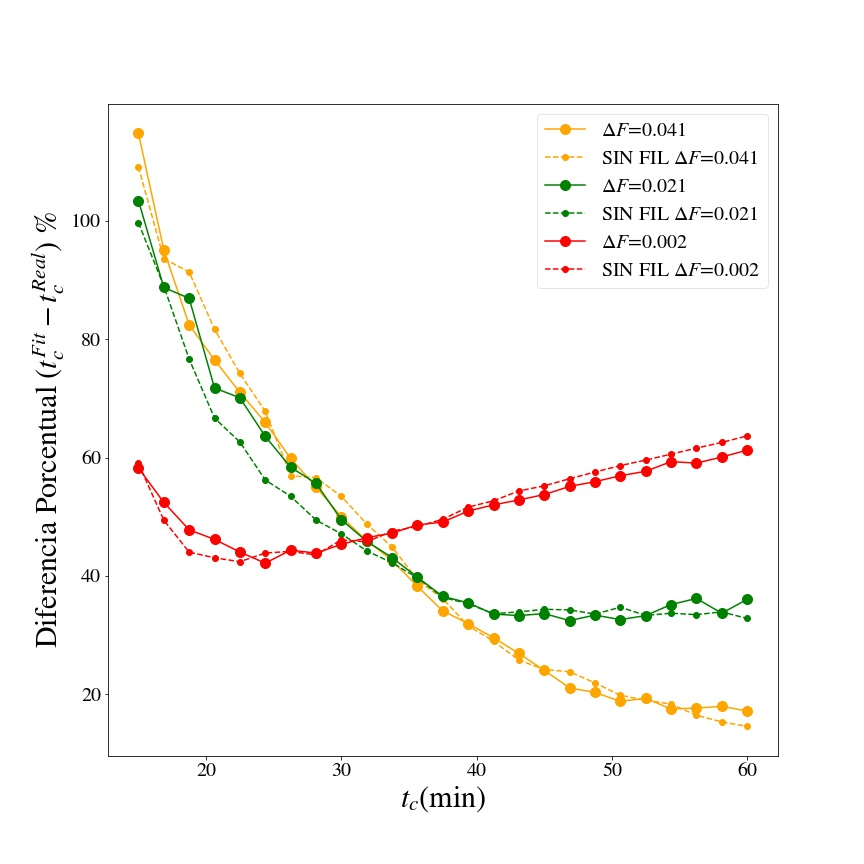
\includegraphics[max size={\textwidth}{0.9\textheight}]{./figures/Dif_SNR_10_Mov.jpg}
		\caption{Las lineas sólidas representan la diferencia porcentual entre $t_{c}^{Fit}$ y $t_{c}^{Real}$ después de aplicar el modelo del trapezoide a los datos filtrados utilizando promedio móvil. Las líneas punteadas representan la misma cantidad, pero obtenida aplicando el modelo del trapezoide a las curvas simuladas sin filtrar. El color representa diferentes valores de $\Delta F$, se utilizaron 4\%, 2\% y 0.2\% representados en amarillo, verde y rojo respectivamente. Estos resultados se obtuvieron a partir de curvas simuladas a las que se les insertó un ruido con una $SNR=10$.}
		\label{fig_diferencias_mov_10}
\end{figure}

\begin{figure}
	\centering
		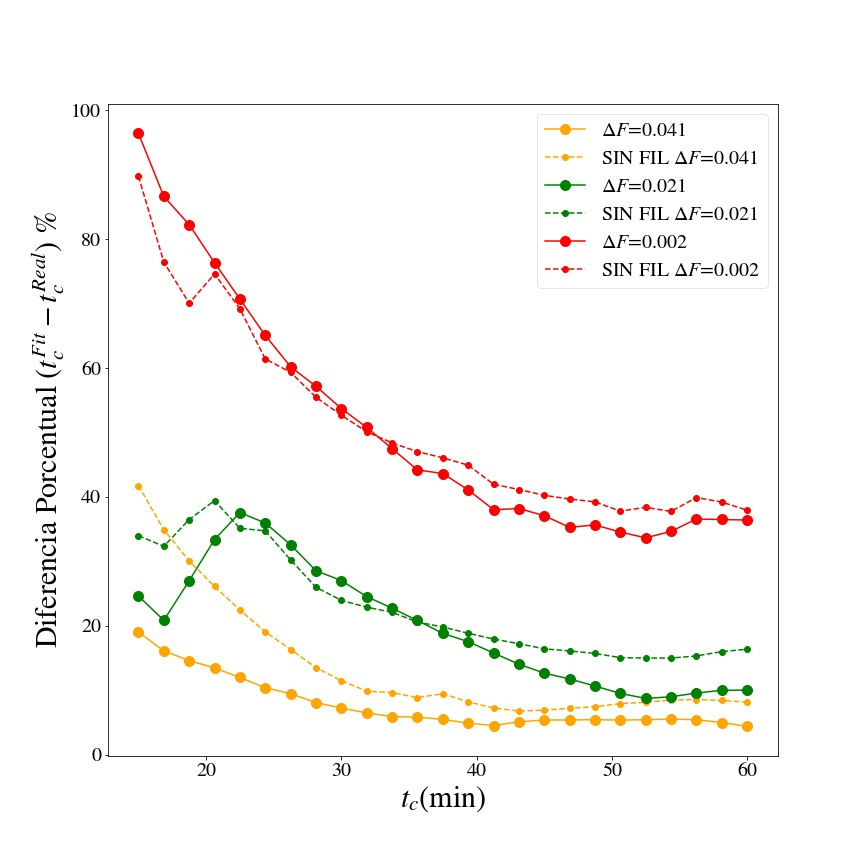
\includegraphics[max size={\textwidth}{0.9\textheight}]{./figures/Dif_SNR_100_Mov.jpg}
		\caption{Las lineas sólidas representan la diferencia porcentual entre $t_{c}^{Fit}$ y $t_{c}^{Real}$ después de aplicar el modelo del trapezoide a los datos filtrados utilizando promedio móvil. Las líneas punteadas representan la misma cantidad, pero obtenida aplicando el modelo del trapezoide a las  curvas simuladas sin filtrar. El color representa diferentes valores de $\Delta F$, se utilizaron 4\%, 2\% y 0.2\% representados en amarillo, verde y rojo respectivamente. Estos resultados se obtuvieron a partir de curvas simuladas a las que se les insertó un ruido con una $SNR=100$}
		\label{fig_diferencias_mov_100}
\end{figure}

Podemos observar que este método es el menos efectivo, si queremos obtener una medida precisa de $t_{c}$. No se aprecia una diferencia significativa entre los resultados para las mismas curvas con y sin filtrar. Esto se debe a lo que se mencionaba con anterioridad, este método altera la forma de la señal inmersa en el ruido. Al promediar en el tiempo, la pendiente de entrada/saluda en la curva de luz cambia (véase \ref{fig_2_2_transito_curva}), esto provoca que aún suavizando la curva y obteniendo un buen coeficiente de correlación, el valor real puede ser diferente del calculado.

Esta deformación parece aumentar de manera proporcional a $t_{c}$. Este método es el menos eficiente computacionalmente hablando.

\subsubsection*{IV.1.1.3 Resultados del filtrado con PCA}
\addcontentsline{toc}{subsubsection}{IV.1.1.3 Resultados del filtrado con PCA}

De manera análoga, las figuras \ref{fig_correlaciones_pca_10} y \ref{fig_correlaciones_pca_100} muestran la correlación, entre el modelo y la curva filtrada con el método de análisis de componentes principales (PCA), para curvas con $SNR=10$ y $SNR=100$ respectivamente. El color nos indica la media de los coeficientes de correlación ($C$), de los 100 ruidos con diferentes parámetros (véase III.2.3).

\begin{figure}[H]
	\centering
		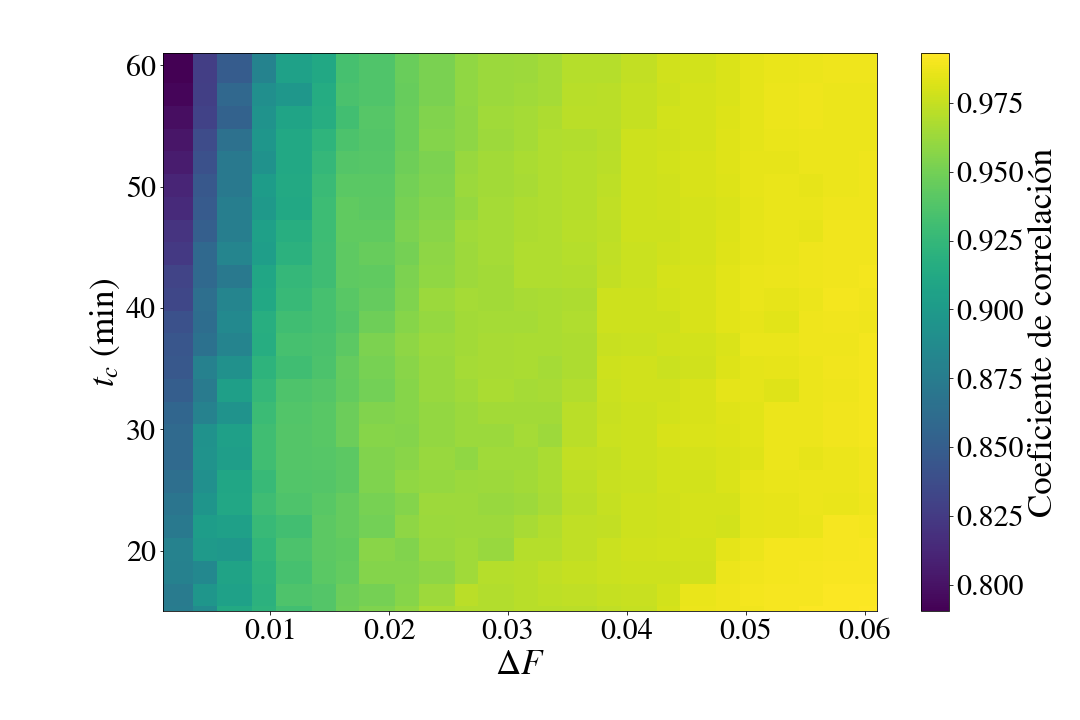
\includegraphics[max size={0.9\textwidth}{0.36\textheight}]{./figures/corrPCASNR_10.png}
		\caption{Matriz de correlaciones de los parámetros $\Delta F$ y $t_{c}$ entre las simulaciones y los calculados después de aplicar el modelo del trapezoide a los datos filtrados utilizando PCA. Estos resultados se obtuvieron a partir de curvas con una $SNR=10$.}
		\label{fig_correlaciones_pca_10}
\end{figure}

\begin{figure}
	\centering
		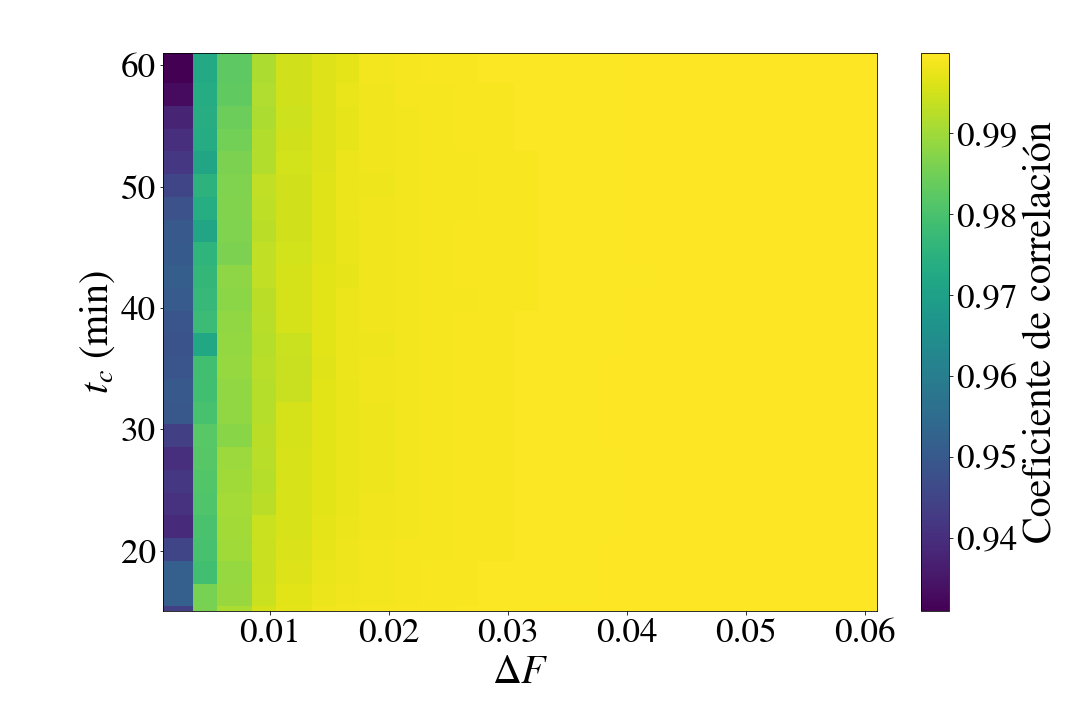
\includegraphics[max size={0.9\textwidth}{0.36\textheight}]{./figures/corrPCASNR_100.png}
		\caption{Matriz de correlaciones de los parámetros $\Delta F$ y $t_{c}$ entre las simulaciones y los calculados después de aplicar el modelo del trapezoide a los datos filtrados utilizando PCA. Estos resultados se obtuvieron a partir de curvas con una $SNR=100$.}
		\label{fig_correlaciones_pca_100}
\end{figure}

El filtrado usando PCA método arroja los coeficientes de correlación más altos, sin embargo lo mismo ocurrió en la prueba de falsos positivos. Para este método, la cota inferior para determinar una curva como candidata a tránsito es de $C \geq 0.94 $. 

Si analizamos las figuras  \ref{fig_correlaciones_pca_10} y \ref{fig_correlaciones_pca_100}, vemos que al igual que para el método de Fourier, no se ve una correlación significativa entre $C$ y $t_{c}$. 

Las figuras \ref{fig_diferencias_pca_10} y \ref{fig_diferencias_pca_100} muestran la diferencia porcentual entre $t_{c}^{Fit}$ y $t_{c}^{Real}$, que representan la duración de $t_{c}$ calculada mediante el ajuste y el valor real de la simulación respectivamente. El color nos indica diferentes valores de $\Delta F$. En la figura \ref{fig_diferencias_pca_10} se ilustra los resultados para una $SNR=10$ y los de $SNR=100$ en la figura \ref{fig_diferencias_pca_100}.

\begin{figure}
	\centering
		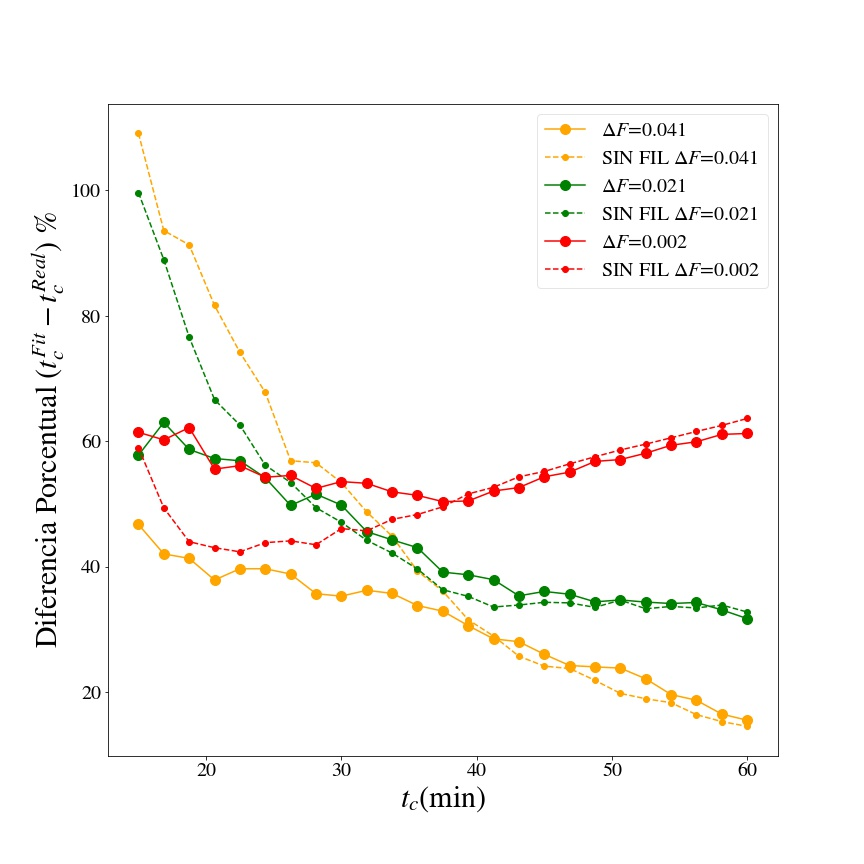
\includegraphics[max size={\textwidth}{0.9\textheight}]{./figures/Dif_SNR_10_PCA.jpg}
		\caption{Las lineas sólidas representan la diferencia porcentual entre $t_{c}^{Fit}$ y $t_{c}^{Real}$ después de aplicar el modelo del trapezoide a los datos filtrados utilizando PCA. Las líneas punteadas representan la misma cantidad, pero obtenida aplicando el modelo del trapezoide a las  curvas simuladas sin filtrar. El color representa diferentes valores de $\Delta F$, se utilizaron 4\%, 2\% y 0.2\% representados en amarillo, verde y rojo respectivamente. Estos resultados se obtuvieron a partir de curvas simuladas a las que se les insertó un ruido con una $SNR=10$.}
		\label{fig_diferencias_pca_10}
\end{figure}

\begin{figure}
	\centering
		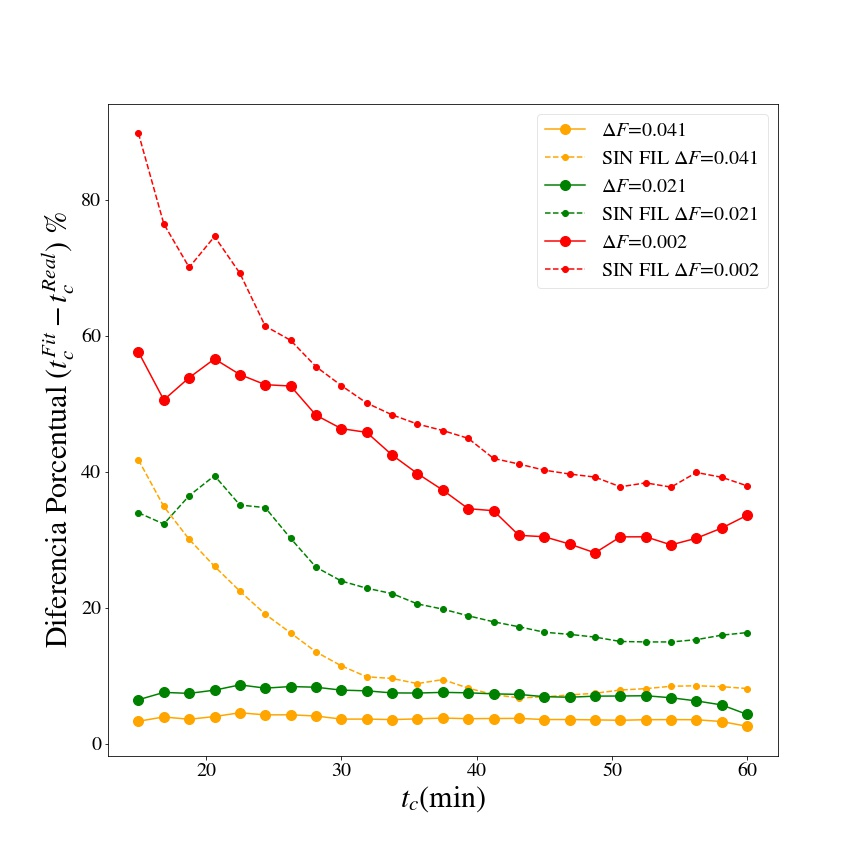
\includegraphics[max size={\textwidth}{0.9\textheight}]{./figures/Dif_SNR_100_PCA.jpg}
		\caption{Las lineas sólidas representan la diferencia porcentual entre $t_{c}^{Fit}$ y $t_{c}^{Real}$ después de aplicar el modelo del trapezoide a los datos filtrados utilizando PCA. Las líneas punteadas representan la misma cantidad, pero obtenida aplicando el modelo del trapezoide a las  curvas simuladas sin filtrar. El color representa diferentes valores de $\Delta F$, se utilizaron 4\%, 2\% y 0.2\% representados en amarillo, verde y rojo respectivamente. Estos resultados se obtuvieron a partir de curvas simuladas a las que se les insertó un ruido con una $SNR=100$}
		\label{fig_diferencias_pca_100}
\end{figure}

Podemos observar que este método es el más efectivo, si queremos obtener una medida precisa de $t_{c}$. De igual manera que el filtro de Fourier, este funciona mejor para pendientes más grandes, es decir tiempos de entrada/salida cortos ($\lesssim 30$ min). Se aprecia una mejora debido al filtrado para todos los valores de $t_{c}$ del al menos 15\%. También cabe destacar que este método de filtrado es el más eficiente, esto desde el punto de vista computacional.

\newpage
\section*{IV.2 Datos observacionales}
\addcontentsline{toc}{section}{IV.2 Datos observacionales}

Se presentan los resultados de las metodologías para la mejora de la SNR en las curvas de luz reales (véase III.1).

\subsection*{IV.2.1 Mejora de la señal a ruido en datos observacionales}
\addcontentsline{toc}{subsection}{IV.2.1 Mejora de la señal a ruido en datos observacionales}

Se le aplico la metodología propuesta en este trabajo a todas las curvas de luz (véase tabla \ref{tab_resultados_obs}, sin embargo por presentación se presentan los resultados del filtrado de ruido en la curva de luz de alta cadencia de HAT-P-37, utilizando las 3 metodologías descritas en la sección anterior: el filtro de frecuencias de Fourier, promedio móvil y análisis de componentes principales (PCA). La curva de luz de HAT-P-37 fue obtenida mediante fotometría de apertura utilizando APPHi.


\begin{figure}[h!]
	\centering
	  \includegraphics[max size={0.9\textwidth}{0.9\textheight}]{./figures/hat37b_sinfil_2.png}
	 \caption{Curva de luz de HAT-P-37b tomada a 20 fps, durante la segunda mitad del tránsito. La curva de luz se obtuvo mediante fotometría de apertura con una $SNR=11.73$. La línea negra representa el modelo teórico, utilizando los parámetros presentados en \cite{bakos2012hat}.}
	  \label{fig_transito_hat37b}
  \end{figure}


\subsubsection*{IV.2.1.1 Resultados del filtro de Fourier}
\addcontentsline{toc}{subsubsection}{IV.2.1.1 Resultados del filtro de Fourier}

En la figura \ref{fig_transito_fou} podemos apreciar el resultado del filtro pasabajas de Fourier, aplicado a la curva de luz de HAT-P-37b. A pesar de ser una curva con mucho ruido, se puede apreciar a simple vista la forma del tránsito. Se utilizó una frecuencia de corte $FC$ de $2\times 10^{-3}$. También se muestra el modelo teórico del tránsito en negro, simulado usando los parámetros presentados en \cite{bakos2012hat} y \textit{BATMAN} (véase III.3.1). La similitud entre el modelo y la curva filtrada es alto, el coeficiente de correlación es de $C=0.982$.

\begin{figure}
	\centering
	  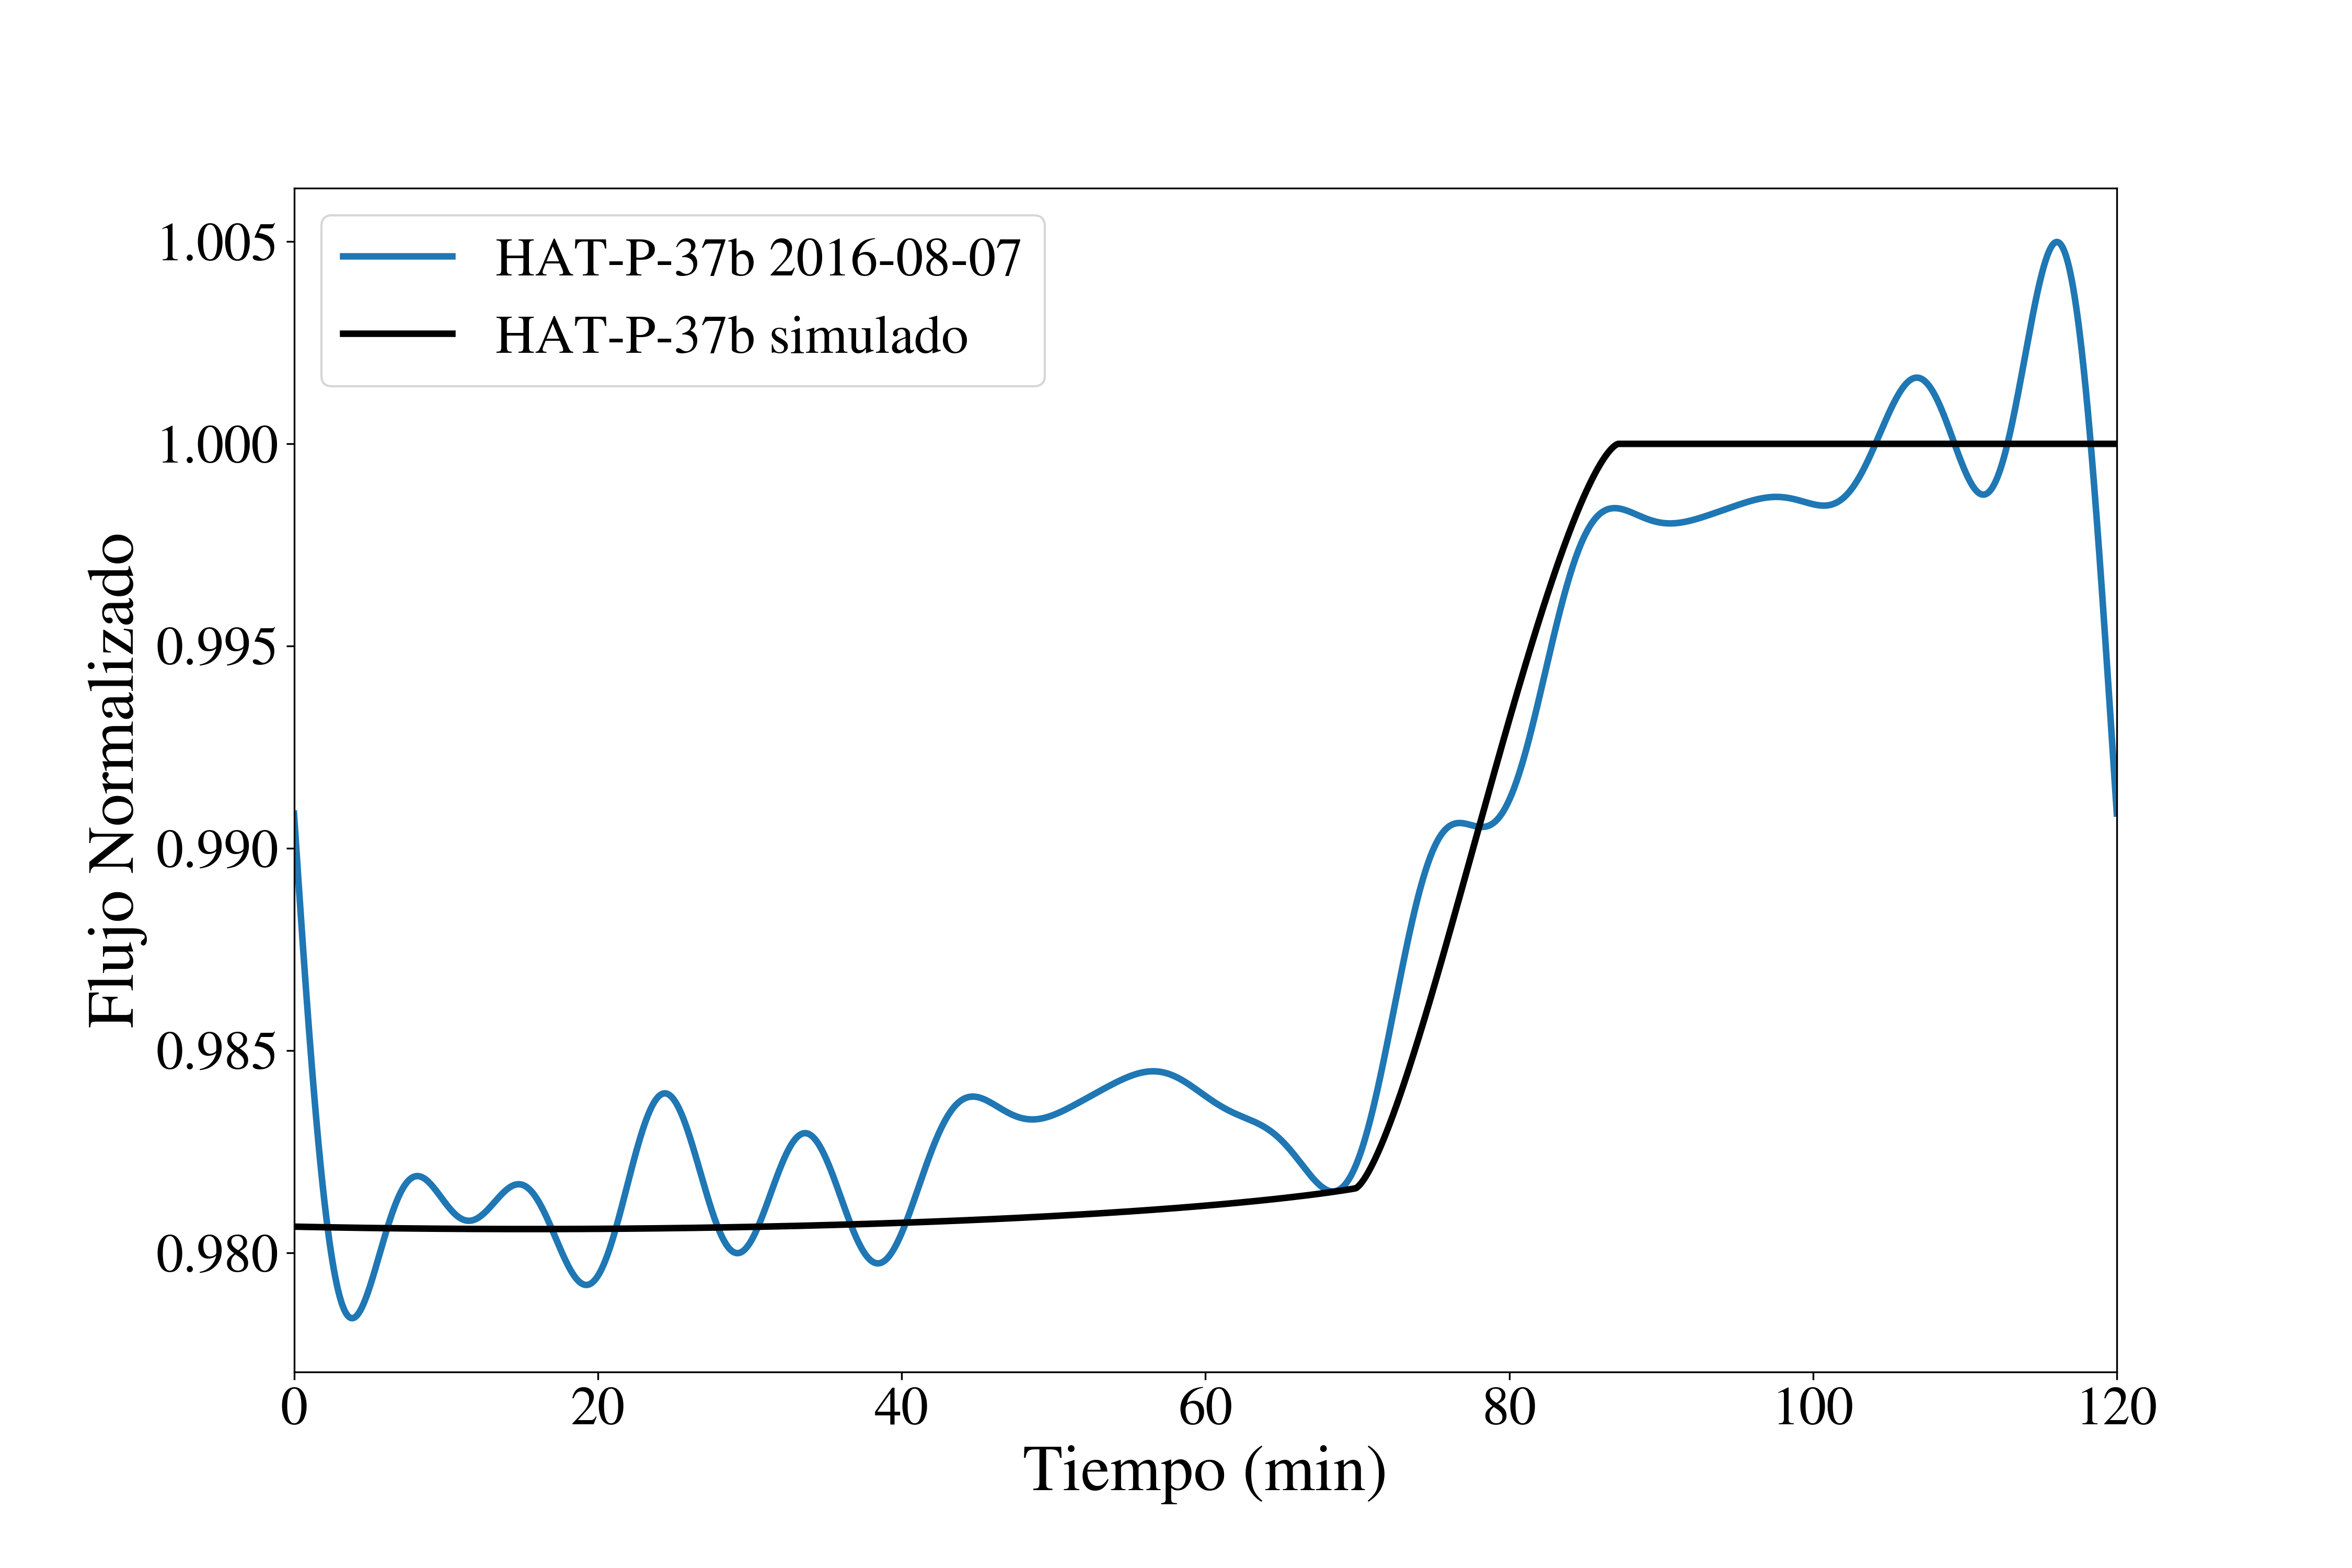
\includegraphics[max size={0.9\textwidth}{0.9\textheight}]{./figures/hat37b_fou_2.png}
	 \caption{Azul: curva de luz de HAT-P-37b después del filtrado de altas frecuencias. La señal a ruido resultante fue de $SNR=124.75$. La línea negra representa el modelo teórico, utilizando los parámetros presentados en \cite{bakos2012hat}. El coeficiente de correlación entre la curva y el modelo es $C=0.982$.}
	  \label{fig_transito_fou}
  \end{figure}

\subsubsection*{IV.2.1.2 Resultados del promedio móvil}
\addcontentsline{toc}{subsubsection}{IV.2.1.2 Resultados del promedio móvil}

En la figura \ref{fig_transito_mov} podemos apreciar el resultado del promedio móvil, aplicado a la curva de luz de HAT-P-37b. Para este resultado, se utilizó una ventana de 3000 frames. De igual manera se muestra en negro el modelo teórico. La similitud entre el modelo y la curva filtrada es alto, el coeficiente de correlación es de $C=0.962$.

\begin{figure}
\centering
	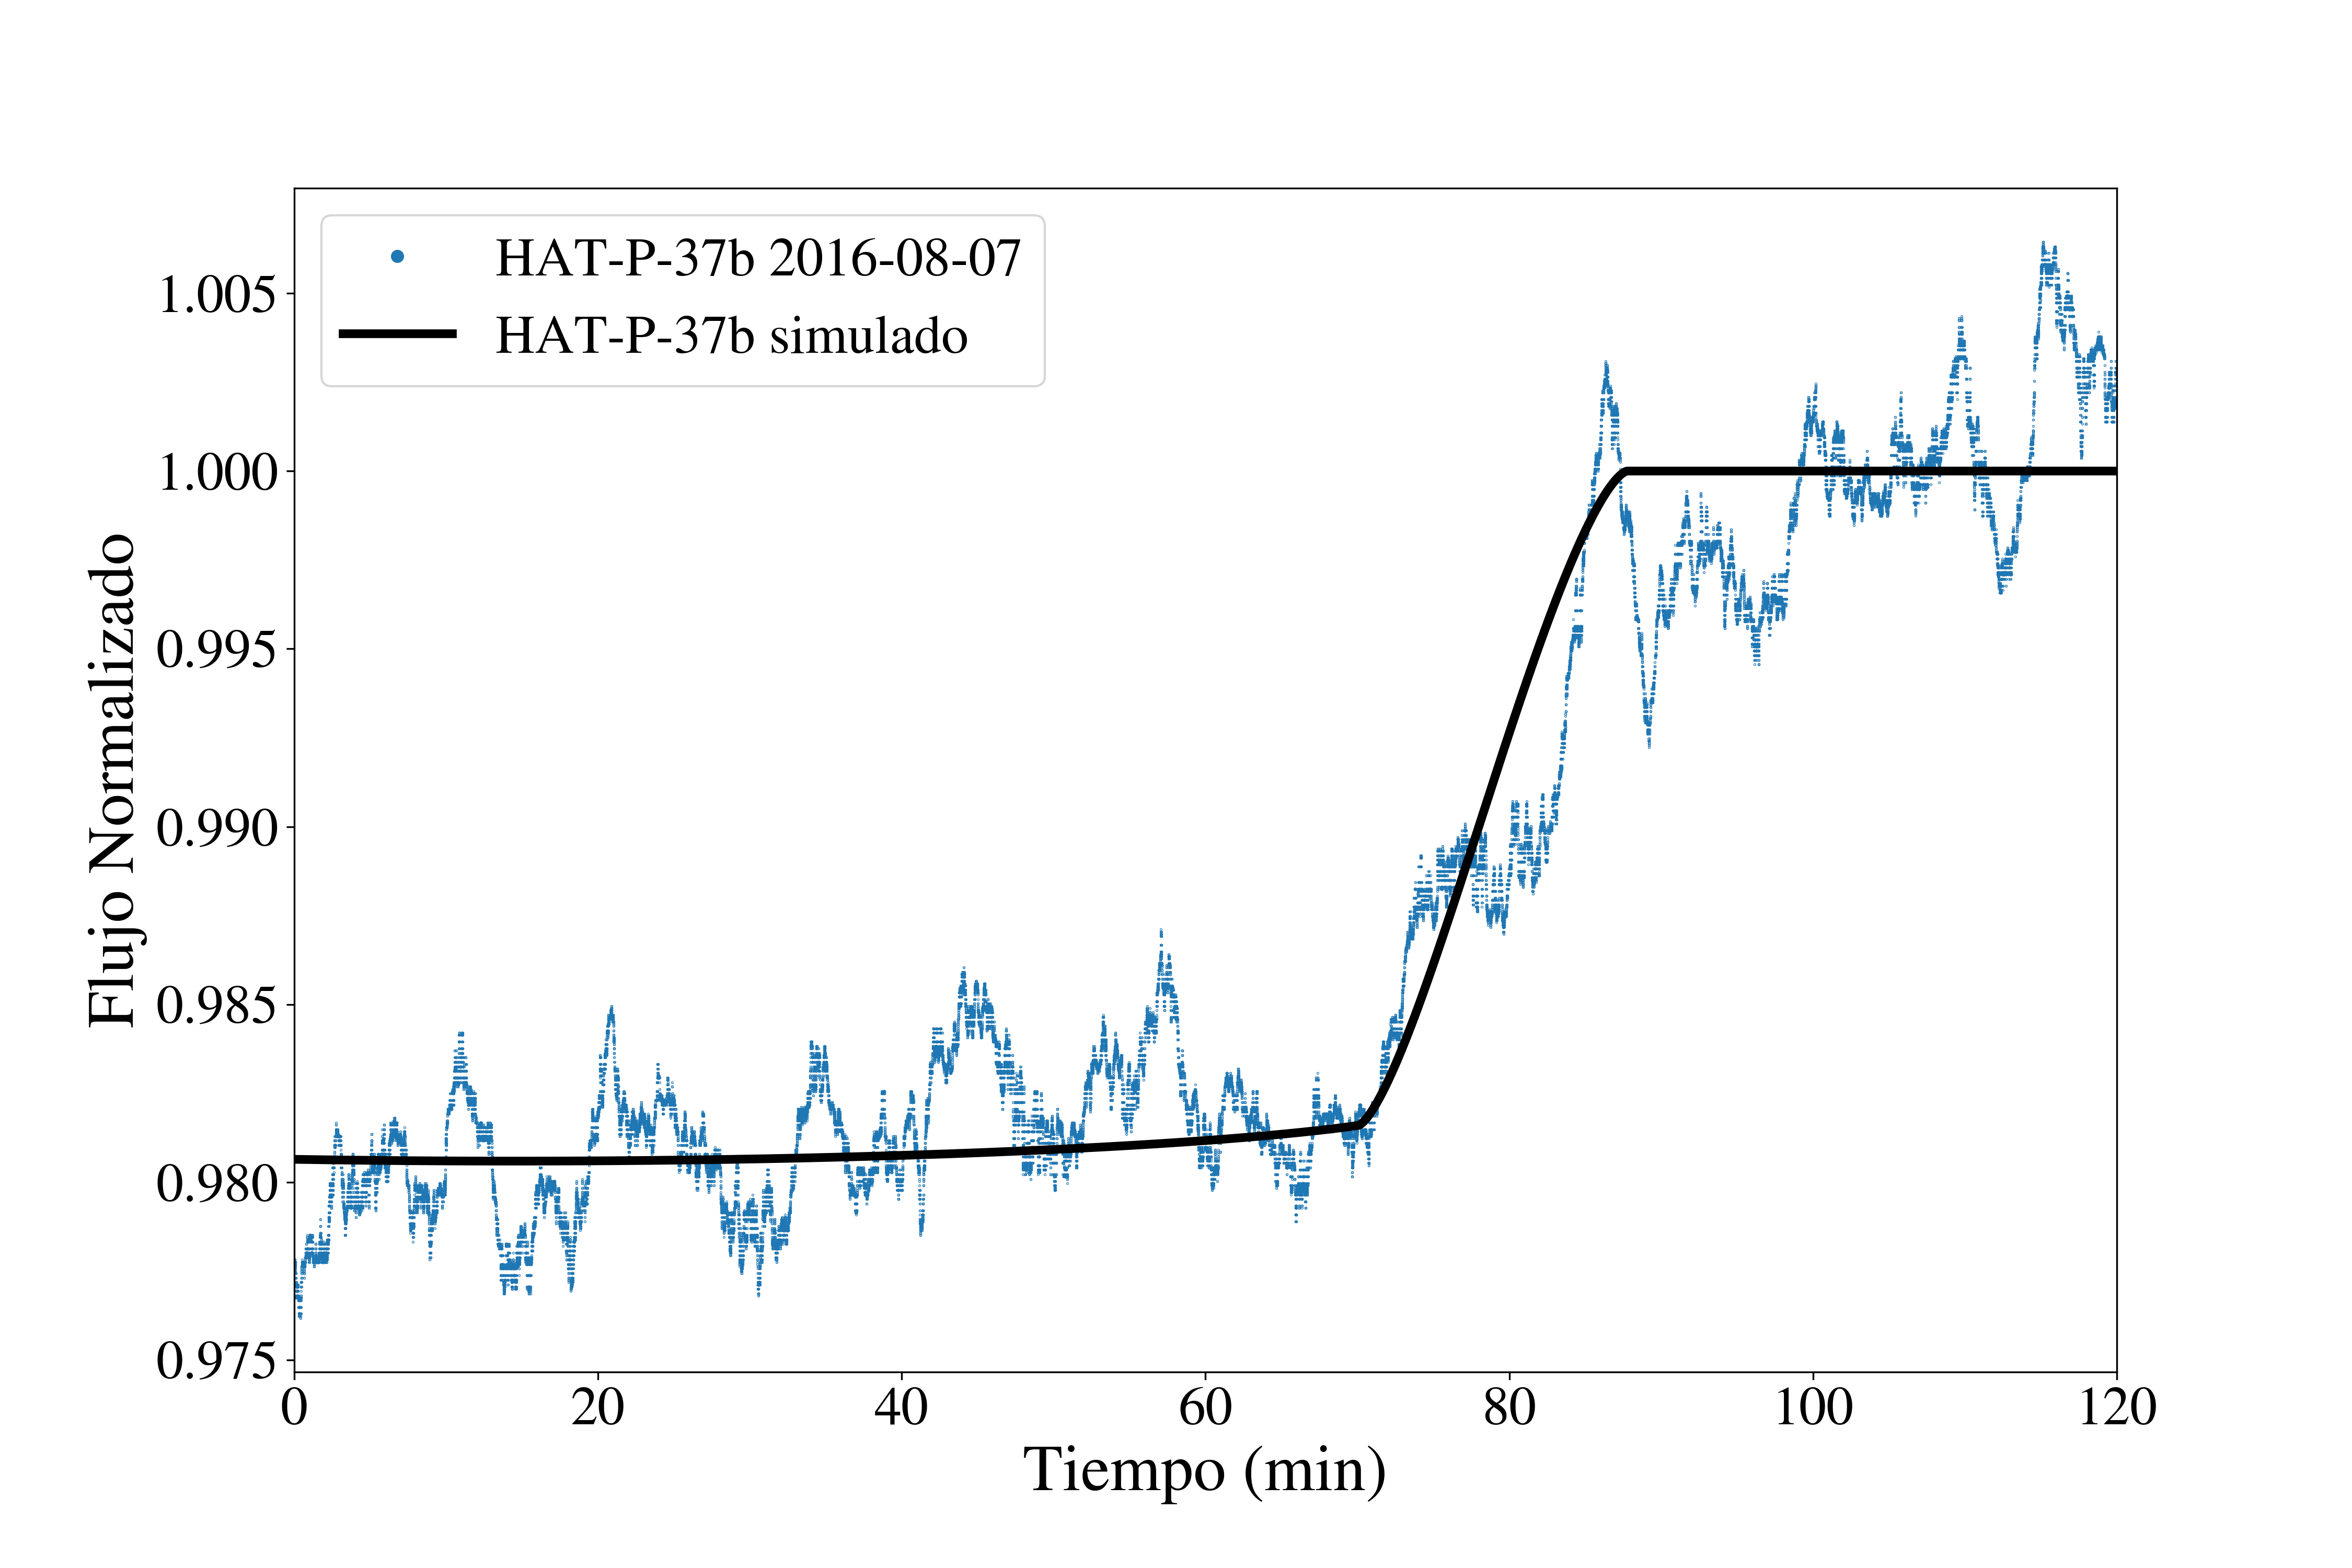
\includegraphics[max size={0.9\textwidth}{0.9\textheight}]{./figures/hat37b_mov_2.png}
	\caption{Azul: curva de luz de HAT-P-37b después del promedio móvil. La señal a ruido resultante fue de $SNR=116.64$. La línea negra representa el modelo teórico, utilizando los parámetros presentados en \cite{bakos2012hat}. El coeficiente de correlación entre la curva y el modelo es $C=0.962$.}
	\label{fig_transito_mov}
\end{figure}

Como se observa en la figura \ref{fig_transito_mov}, este método altera la pendiente de la curva, donde el planeta está saliendo de la superficie solar. Esta deformación es proporcional a la longitud de la ventana de promediado, por lo que ventanas pequeñas (1000-3000 frames) pueden dar mejores coeficientes de correlación. 


\subsubsection*{IV.2.1.3 Resultados de PCA}
\addcontentsline{toc}{subsubsection}{IV.2.1.3 Resultados del PCA}

En la figura \ref{fig_transito_pca} podemos apreciar el resultado del filtrado utilizando el análisis de componentes principales (PCA), aplicado a la curva de luz de HAT-P-37b. Se calcularon las componentes principales de un conjunto de 25 tránsitos simulados con diferentes $\Delta F$ y $t_{c}$. Debido a que la componentes principales son calculadas utilizando una variedad de parámetros, la curva resultado solo posee la forma de tránsito, sin embargo, no es ideal para ser utilizada para el cálculo de observables.

\begin{figure}
	\centering
		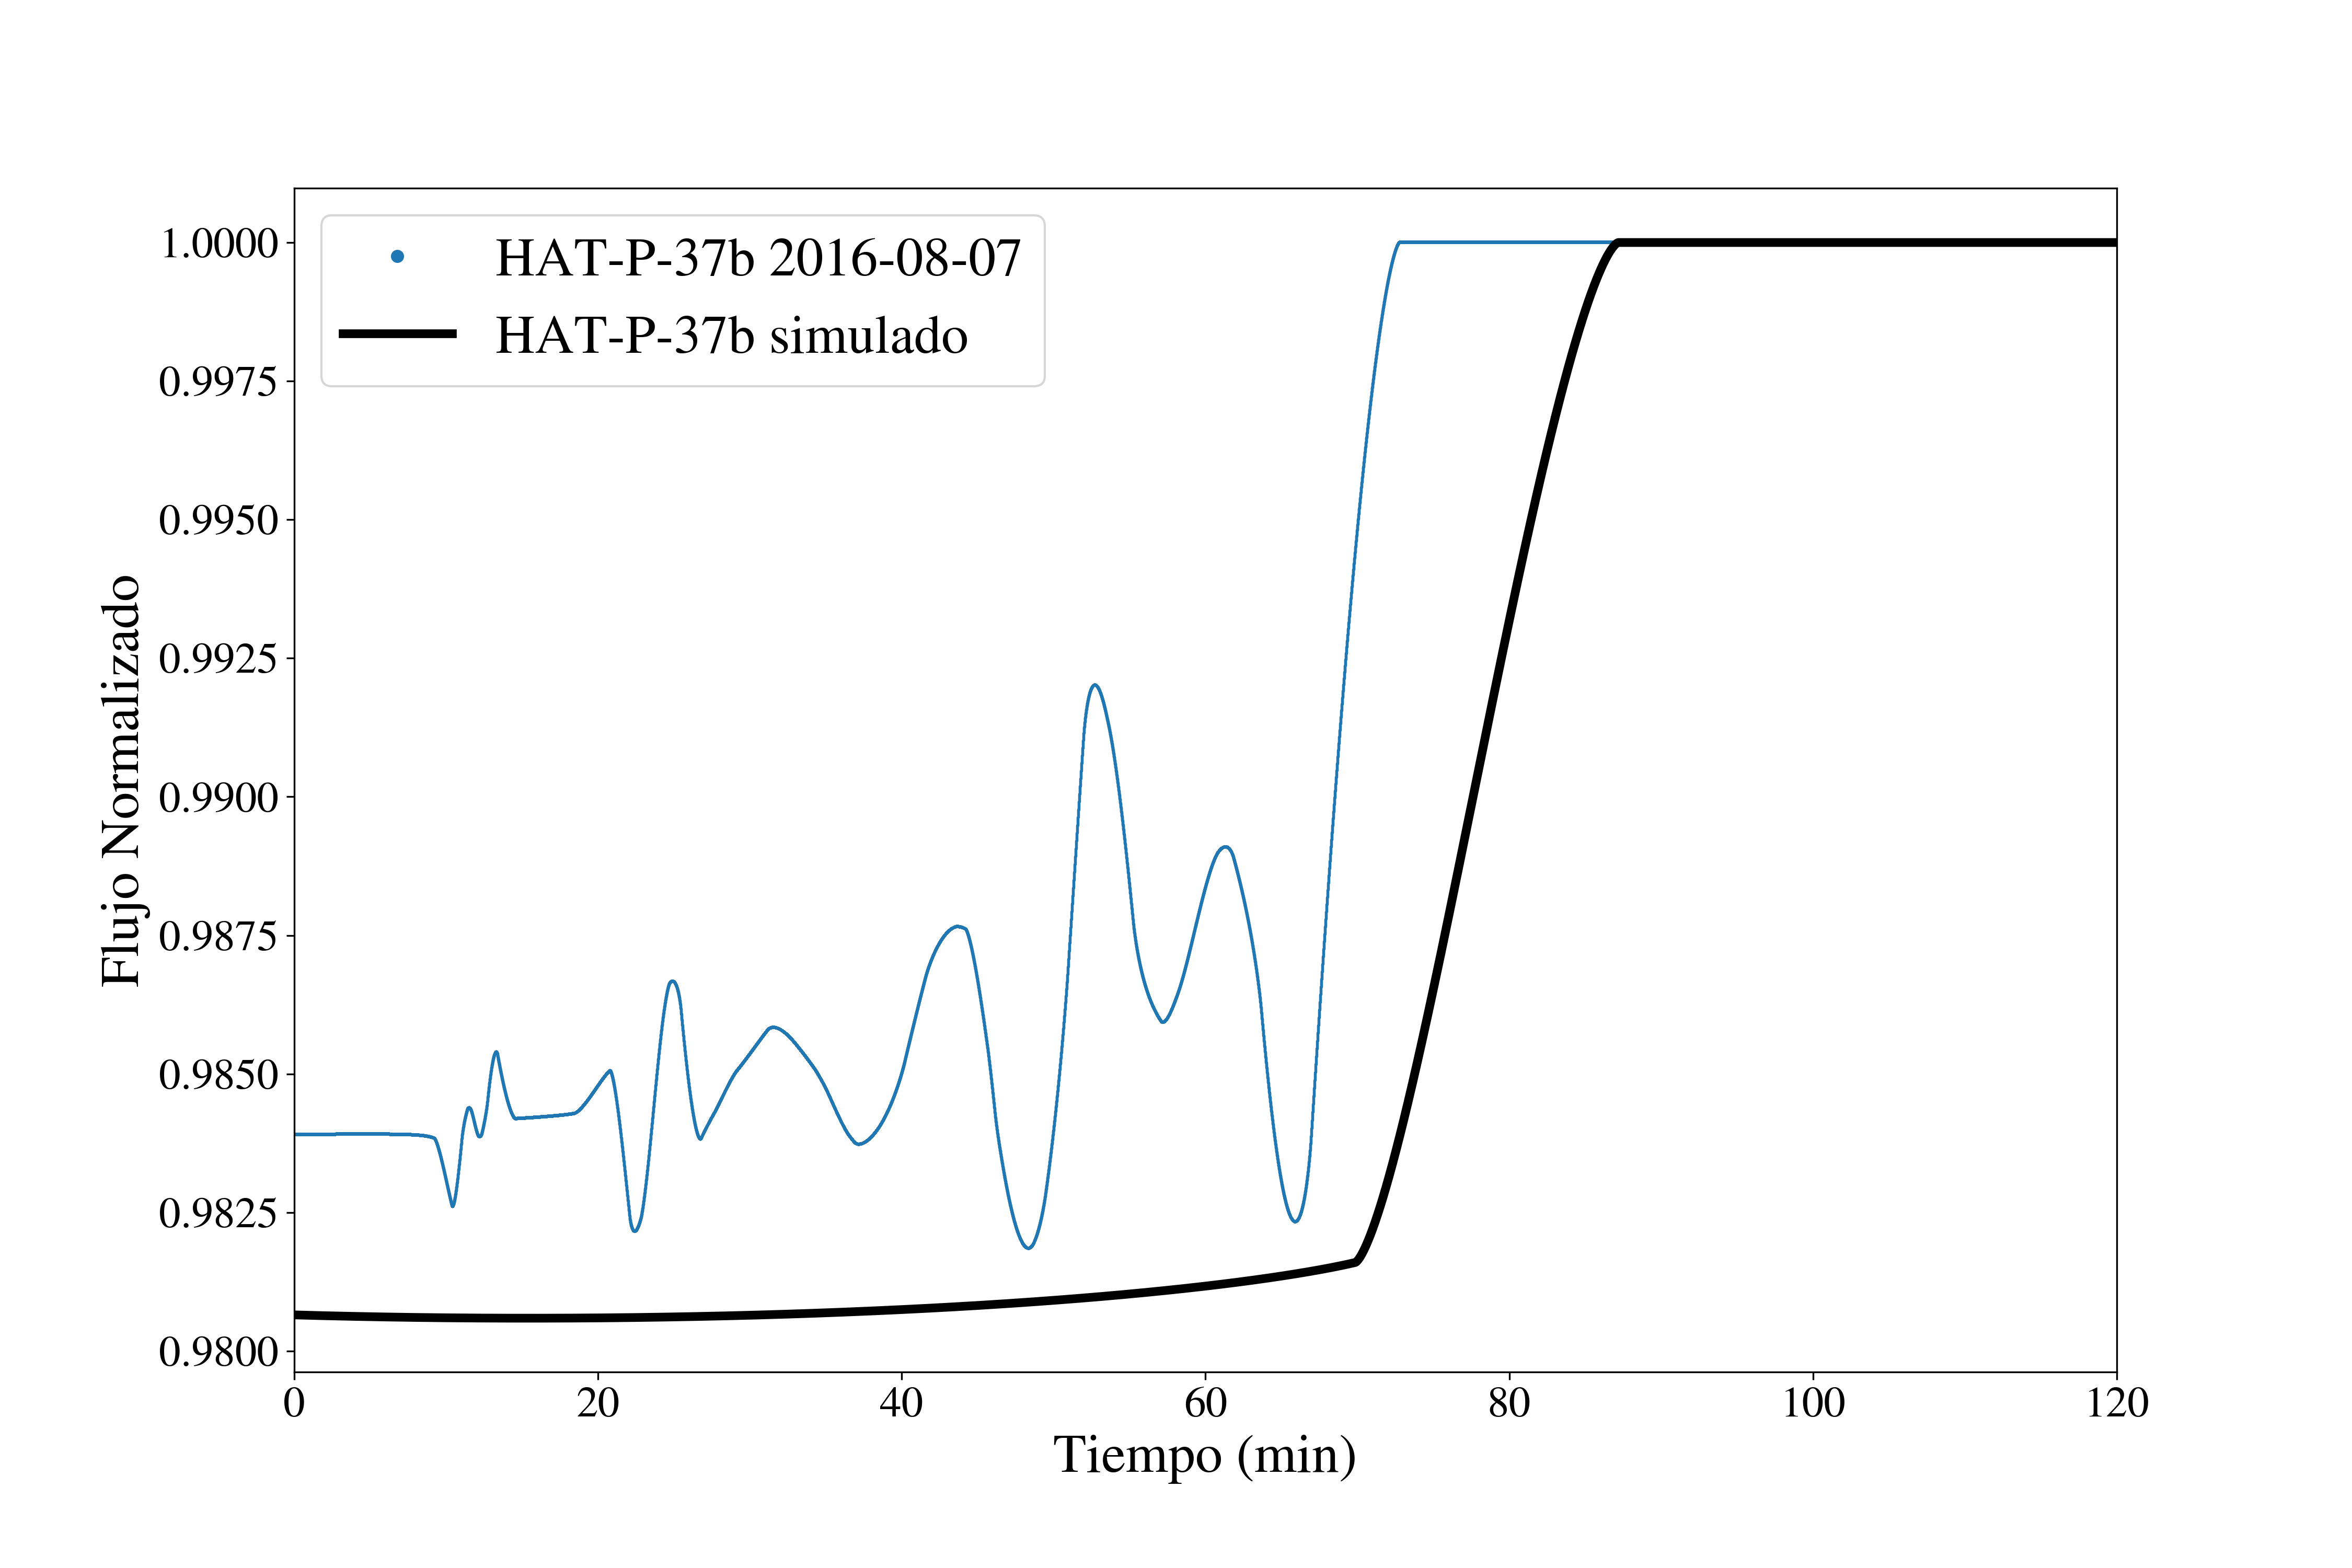
\includegraphics[max size={0.9\textwidth}{0.9\textheight}]{./figures/hat37b_pca_2.png}
		\caption{Azul: curva de luz de HAT-P-37b después del filtrado con PCA. La señal a ruido resultante fue de $SNR=135.51$. La línea negra representa el modelo teórico, utilizando los parámetros presentados en \cite{bakos2012hat}. El coeficiente de correlación entre la curva y el modelo es $C=0.889$.}
		\label{fig_transito_pca}
\end{figure}

Esta metodología funciona para la visualización, y como método de comparación entre los modelos teóricos y las curvas de luz. Si las curva de luz, contiene componentes principales similares a las del modelo, se producirá una curva similar a la que se observa en la figura \ref{fig_transito_pca}. Si la curva es solo ruido, el resultado será una curva errática sin ningún parecido con el modelo como se muestra en la figura \ref{fig_puro_ruido_pca}.

\begin{figure}
	\centering
		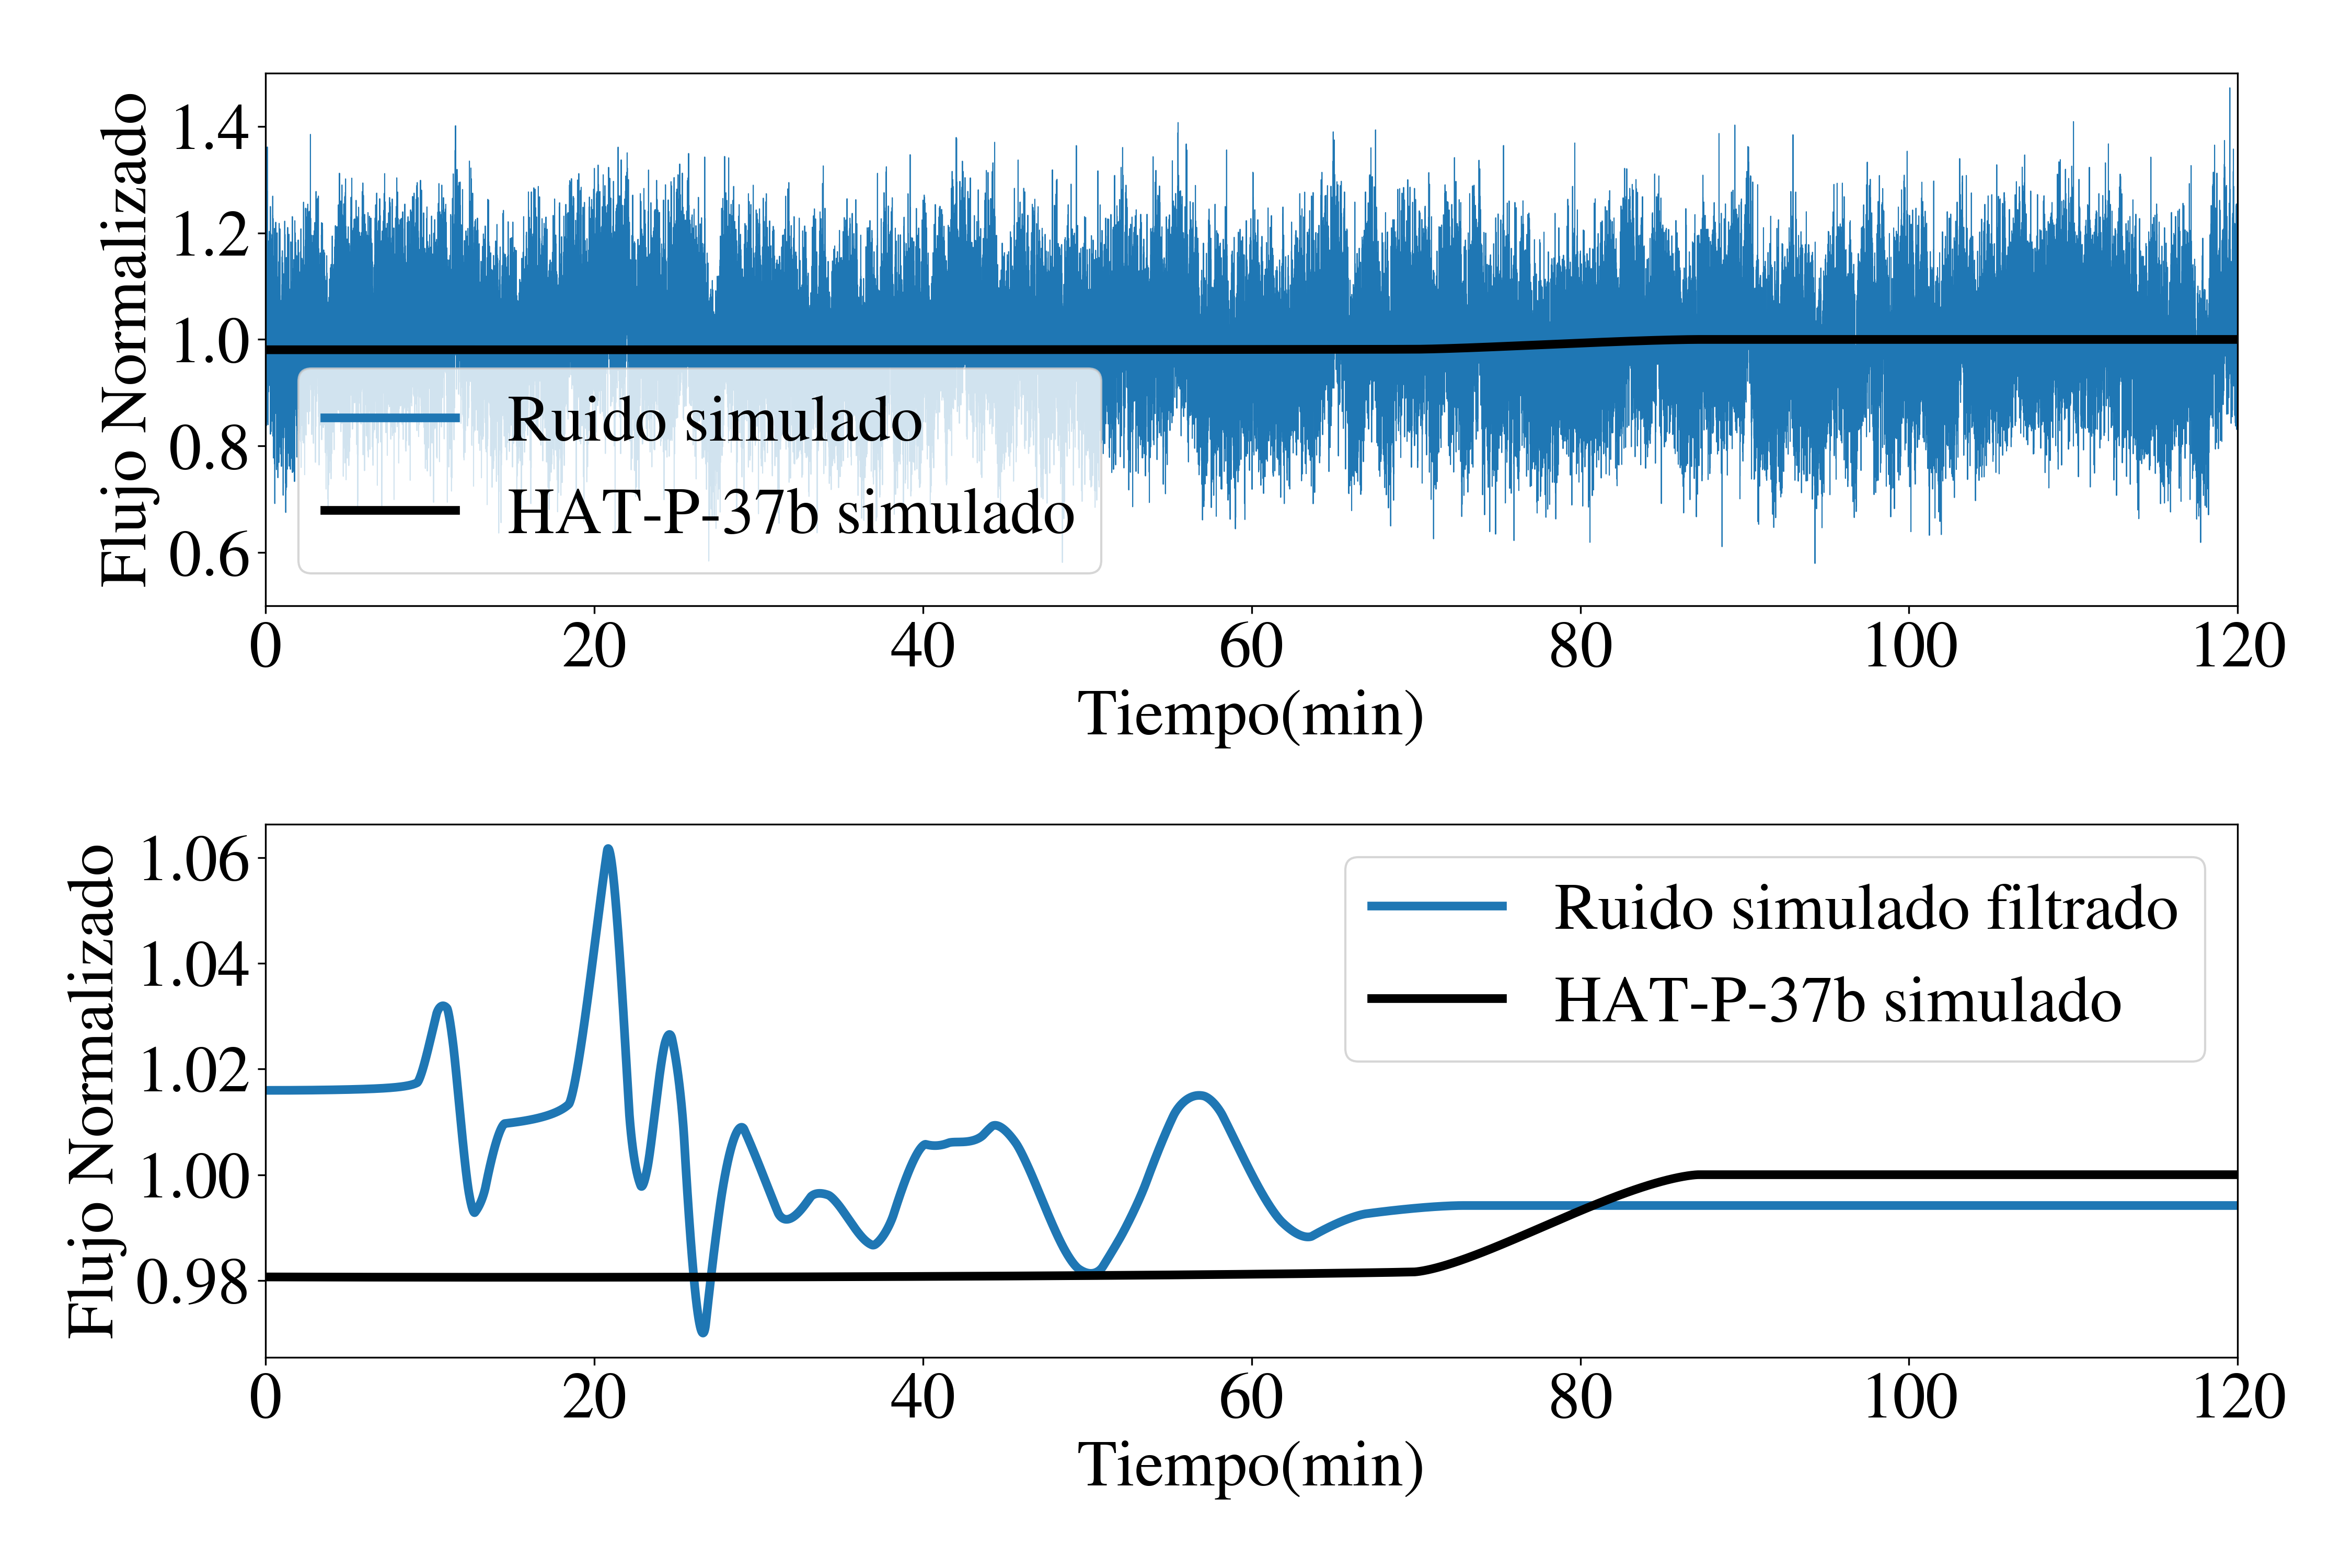
\includegraphics[max size={\textwidth}{\textheight}]{./figures/PCA_puro_ruido.png}
		\caption{Arriba: Ruido simulado con componentes de baja frecuencia en su espectro. La línea negra representa el modelo teórico de HAT-P-37b, utilizando los parámetros presentados en \cite{bakos2012hat}. Abajo: en azul se muestra el resultado de PCA a una curva sin tránsito inmerso.}
		\label{fig_puro_ruido_pca}
\end{figure}


\newpage
\subsubsection*{IV.2.1.4 Resumen de resultados con datos observacionales}
\addcontentsline{toc}{subsubsection}{IV.2.1.4 Resumen de resultados con datos observacionales}

En la tabla \ref{tab_resultados_obs} se presentan todos los resultados de la mejora de la SNR utilizando las metodologías descritas anteriormente, para todo el conjunto de curvas de luz reales (véase III.1)

\begin{table}[h!]
	\centering
	\begin{tabular}{ccccccccc}
	\hline 
	Fecha & Nombre & SNR & $\mbox{SNR}_{Fourier}$ &  $\mbox{SNR}_{mov}$ & $\mbox{SNR}_{PCA}$\\ 
	\hline
	06/Ago/2016 & WASP-74b$^{1}$ & 47.03 & 226.50 & 212.93 & 279.51 \\ 
	06/Ago/2016 & WASP-74b$^{2}$ & 39.82 & 114.47 & 114.73 & 156.30 \\
	06/Ago/2016 & HAT-P-32b & 14.55 & 29.68 & 29.43 & 31.85 \\
	07/Ago/2016 & HAT-P-37$^{1}$ & 11.66 & 176.44 & 166.00 & 180.11 \\ 
	07/Ago/2016 & HAT-P-37$^{2}$ & 11.73 & 124.75 & 116.64 & 135.51 \\ 
	28/May/2017 & HAT-P-14b & 61.40 & 154.80 & 158.96 & - \\ 
	29/May/2017 & WASP-74b & 9.46 & 93.33 & 82.86 & 93.86 \\
	31/May/2017 & WASP-48b & 7.74 & 61.25 & 48.16 & 63.29 \\  
	31/May/2017 & WASP-74b & 14.70 & 41.36 & 42.60 & 47.97 \\
	02/Jun/2017 & WASP-48b$^{1}$ & 11.07 & 28.10 & 22.91 & 32.71 \\
	02/Jun/2017 & WASP-48b$^{2}$ & 7.67 & 20.37 & 14.78 & 20.32 \\
	05/Jun/2017 & HAT-P-31b & 6.17 & 68.05 & 43.67 & 80.09 \\
	08/Jun/2018 & Kepler-17b & 146.52 & 523.31 & 512.25 & 602.00 \\ 
	\hline 
	\end{tabular} 
	\caption{Resumen de los resultados para mejorar la SNR en las curvas de luz de tránsitos de exoplanetas obtenidas en múltiples temporadas en el OAN-SPM. SNR indica el valor de ruido después de la fotometría. $\mbox{SNR}_{Fourier}$, $\mbox{SNR}_{mov}$ y $\mbox{SNR}_{PCA}$ indican el valor de ruido resultado del filtrado de Fourier, promedio móvil y PCA respectivamente. Los superíndices indican que la misma curva se dividió en 2 segmentos de 2 horas cada uno, los cuales se analizaron de manera independiente.}
	\label{tab_resultados_obs}
	\end{table}

Todas las curvas de luz de la tabla \ref{tab_resultados_obs} tienen una duración de 2 horas y fueron obtenidas al momento del tránsito de exoplanetario. En la mayoría de las ocasiones, solo se observó la entrada o salida del exoplaneta al disco solar, las curvas con el superíndices ($^{1,2}$) indican que se observó el tránsito completo y se separó en segmentos de 2 horas para su análisis, donde ($^{1}$ y $^{2}$) indican el comienzo y el final del tránsito respectivamente.

\subsection*{IV.2.2 Determinación de candidatos a tránsitos}
\addcontentsline{toc}{subsection}{IV.2.2 Determinación de candidatos a tránsitos}

Cabe destacar que las técnicas de filtrado utilizadas para la mejora de la SNR, deforman la curva de luz, por lo que no es posible recuperar la curva exacta del tránsito. Sin embargo, el objetivo es encontrar variaciones en el flujo, para determinar si la estrella observada puede ser candidata a tener un exoplaneta.

Se aplicó un ajuste del modelo trapezoidal (véase III.6.1) a las curvas filtradas. El desempeño de los distintos método de filtado, se evaluó utilizando el valor de $\Delta F$ resultado del ajuste a los datos filtrados y comparándolo con el valor reportado por la comunidad en bases de datos como \href{http://var2.astro.cz/ETD/index.php}{\textit{Exoplanet Transit Database}}. Estos resultados se aprecian en la tabla \ref{tab_resultados_profundidad}.


\begin{table}
	\centering
	\begin{tabular}{ccccccccc}
	\hline 
	Fecha & Nombre & $\Delta F$ (\%) & $\Delta F_{Fourier}$ (\%) &  $\Delta F_{mov}$ (\%) & $\Delta F_{PCA}$ (\%) \\ 
	\hline
	06/Ago/2016 & WASP-74b$^{1}$ & 1.04 & - & - & - \\ 
	06/Ago/2016 & WASP-74b$^{2}$ & 1.04 & - & - & - \\
	06/Ago/2016 & HAT-P-32b$^{1}$ & 2.44 & - & - & - \\
	07/Ago/2016 & HAT-P-37$^{1}$ & 2.04 & 1.63 & 1.67 & 1.75 \\ 
	07/Ago/2016 & HAT-P-37$^{2}$ & 2.04 & 1.74 & 1.84 & 1.91 \\ 
	28/May/2017 & HAT-P-14b$^{1}$ & 0.5 & - & - & - \\ 
	29/May/2017 & WASP-74b$^{2}$ & 1.04 & 2.42 & 2.59 & 1.62 \\ 
	31/May/2017 & WASP-48b$^{2}$ & 1.0 & - & - & - \\  
	31/May/2017 & WASP-74b$^{1}$ & 1.04 & 6.47 & 6.28 & 6.59 \\
	02/Jun/2017 & WASP-48b$^{1}$ & 1.0 & 6.63 & 5.33 & 7.5 \\
	02/Jun/2017 & WASP-48b$^{2}$ & 1.0 & - & - & - \\
	05/Jun/2017 & HAT-P-31b$^{1}$ & 1.23 & - & - & - \\
	08/Jun/2018 & Kepler-17b$^{1}$ & 2.13 & - & - & - \\ 
	\hline 
	\end{tabular} 
	\caption{Resultados de $\Delta F$ obtenidos ajustando el modelo del trapezoide a las curvas de luz de tránsitos. $\Delta F_{Fourier}$, $\Delta F_{mov}$ y $\Delta F_{PCA}$ representan el valor de $\Delta F$ obtenido después del filtrado de Fourier, promedio móvil y PCA respectivamente. El superíndice $^{1}$ indica que a curva de luz fue obtenida mediante el inicio del tránsito y $^{2}$ indica que la curva contenía el final del tránsito.}
	\label{tab_resultados_profundidad}
	\end{table}

El ajuste trapezoidal, nos regresa como resultado dos parámetros, $\Delta F$ y $t_{c}$ (véase II.1.1). En estos resultados evaluamos solamente el valor de $\Delta F$, esto nos brinda información sobre la magnitud del cambio en el flujo de la estrella observada, el cual es uno de los principales criterios para la selección de un posible candidato a tránsito. 

Los signos (-) en la tabla \ref{tab_resultados_profundidad}, indican que el método de ajuste falló. Esto ocurre cuando el ajuste del modelo nos da como resultado un valor de $\Delta F$ fuera de los límites permitidos. Esto nos indica que la detectabilidad en los datos observacionales fue baja (38\%), en la mayoría de los casos negativos, las curvas de luz tenían tendencias de baja frecuencia después del proceso de fotometría. En la figura \ref{fig_comp_espectros_resultados} comparamos 2 espectros, el primero pertenece a la curva de luz de WASP-74b del 06 de agosto y el de HAT-P-37b del 07 de agosto del 2016.

\begin{figure}
	\centering
		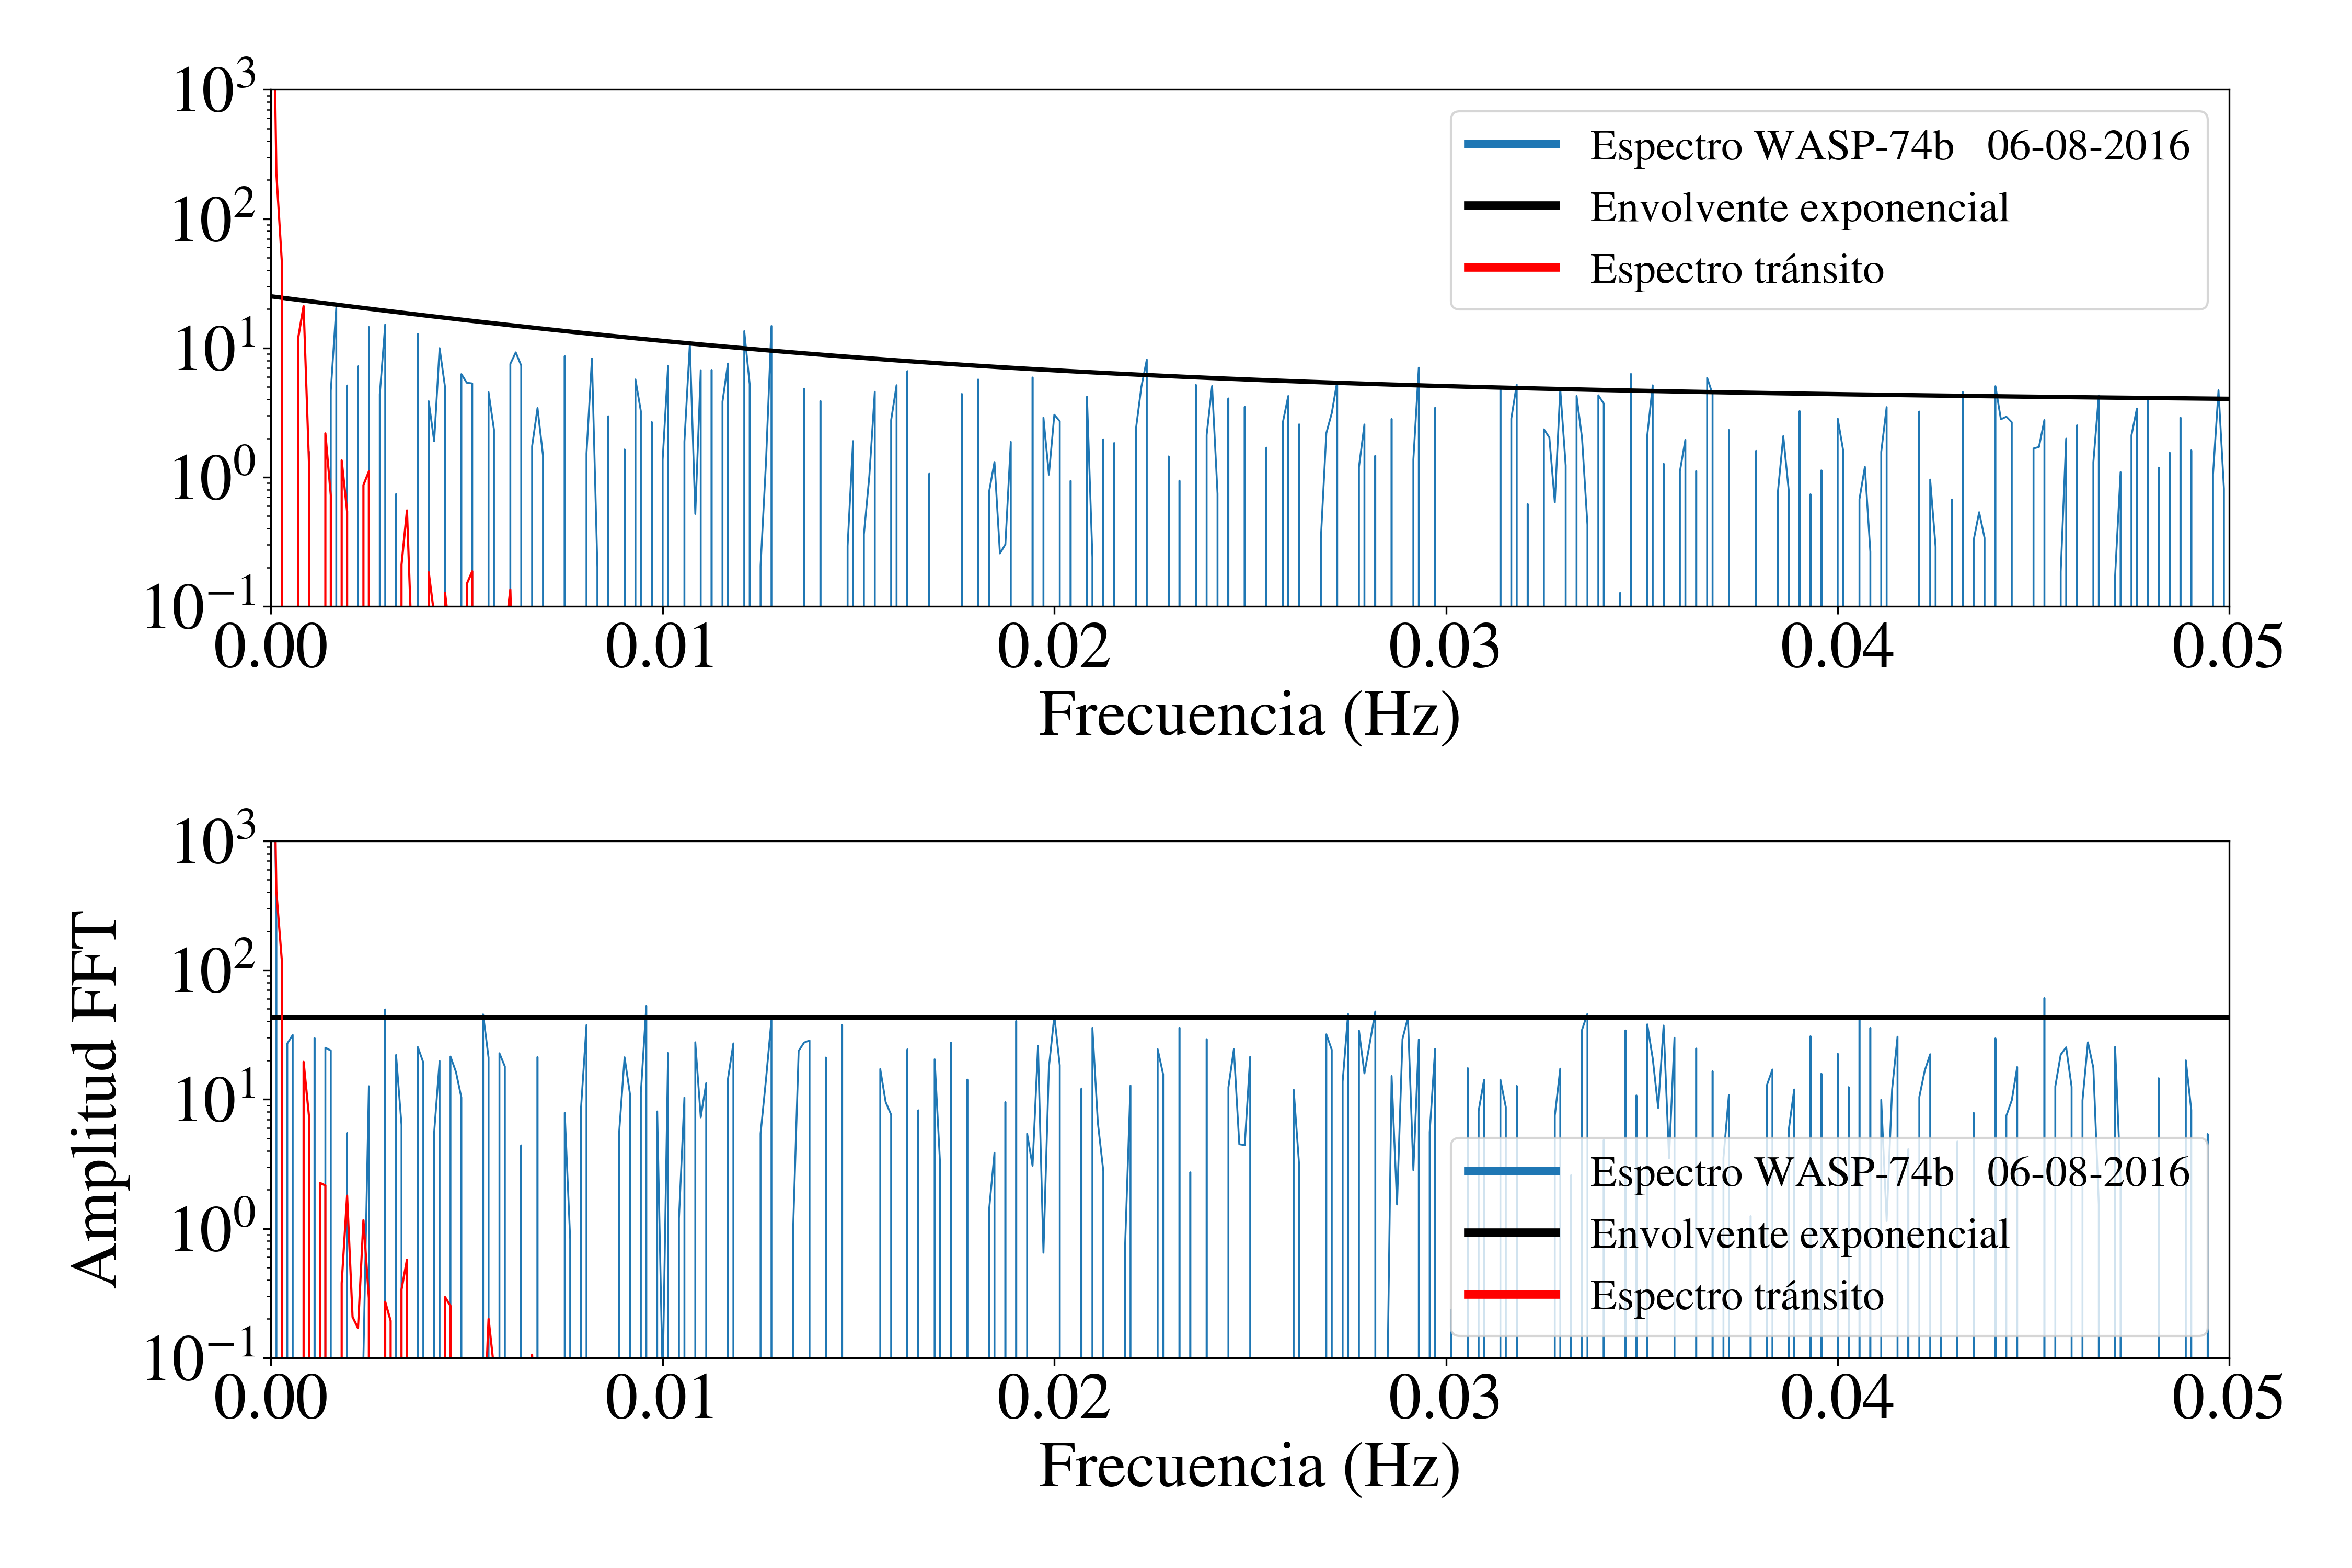
\includegraphics[max size={\textwidth}{\textheight}]{./figures/comparacion_espectros_resultados.png}
		\caption{Arriba: Espectro de la curva de luz de WASP-74b del 06 de agosto. Abajo: Espectro de la curva de luz de HAT-P-37b del 06 de agosto. La línea roja es el espectro del tránsito simulado utilizando los parámetros presentados en \cite{bakos2012hat}. La línea negra representa la envolvente exponencial del espectro. }
		\label{fig_comp_espectros_resultados}
\end{figure}


Comparamos estos espectros, para ilustrar la diferencia entre las curvas en donde el método funciona correctamente (HAT-P-37$^{2}$) y en las que no (WASP-74b$^{1}$) véase tabla \ref{tab_resultados_profundidad}. Podemos apreciar 2 notables diferencias: el nivel de ruido y la envolvente del espectro. El nivel de ruido en la curva de luz HAT-P-37b$^{2}$ es mayor que en la de WASP-74b$^{1}$, esto puede observarse en la tabla \ref{tab_resultados_obs}. Por lo tanto, la SNR en la curva de luz no juega un papel crucial para que el método funcione. Por otra parte, vemos que la envolvente exponencial del espectro de  WASP-74b$^{1}$ posee significativas contribuciones de baja frecuencia, mientras que el espectro de HAT-P-37b$^{2}$ es completamente plano. Esto también puede apreciarse en la tabla \ref{tab:parametros_exponencial}, existe una correlación entre la magnitud de los parámetros ($a_{1},a_{2}$) y los fallos en la identificación de los tránsitos. Cuando la región de bajas frecuencias (línea roja en \ref{fig:3.8_wasp-74b-curva}) se encuentra contaminada, es muy difícil recuperar la señal del tránsito inmersa en el ruido.

En algunos casos como WASP-48b$^{1}$ y HAT-P-31b$^{1}$, las curvas de luz poseen variaciones sistemáticas posiblemente causadas por el movimiento del telescopio. Creemos que en los otros casos fallidos las contribuciones de baja frecuencia fueron causadas al cambio en la masa de aire o al \textit{seeing} de la noche de observación, para mayor detalle véase \cite{guerrero2020effects}, en donde se estudia a detalle este fenómeno y utilizan algunas de las imágenes que utilizamos en este trabajo.